\documentclass[a4paper,10pt]{beamer}
\usepackage[utf8]{inputenc}
\usepackage{color}
\usepackage{colortbl}
\usepackage{xcolor}
\usepackage{caption}
\usepackage{graphicx}
\usepackage{ragged2e}
\usepackage{hyperref}
\usepackage{marvosym}
\usepackage{mathtools}
\usepackage{mdframed}
\usepackage{hologo}
\usepackage{lmodern}
\renewcommand{\figurename}{Figura}
\usetheme{Warsaw}

\def\@fnsymbol#1{\ensuremath{\ifcase#1\or \dagger\or \ddagger\or
   \mathsection\or \mathparagraph\or \|\or **\or \dagger\dagger
   \or \ddagger\ddagger \else\@ctrerr\fi}}%
\renewcommand\thefootnote{\fnsymbol{footnote}}   
\renewcommand\thempfootnote{\fnsymbol{mpfootnote}}
\makeatother

%Borra el footer 
\setbeamertemplate{footline}{}

%Enumerar figuras
\setbeamertemplate{caption}[numbered]

%Alternativa a framebreak	
\newcounter{tmp}
\newcommand\savecounter{\setcounter{tmp}{\value{enumi}}}
\newcommand\continuecounter{\setcounter{enumi}{\value{tmp}}}

%Borra cabecera
\setbeamertemplate{headline}{}


\logo{
\includegraphics[scale=0.05]{logoUNAM}}

\begin{document}

\begin{frame}
\Large
\title{Tubos fotomultiplicadores (FM) y fotodiodos}
\author{Favio Vázquez\footnote{favio.vazquezp@gmail.com}}
\institute{Instituto de Ciencias Nucleares - UNAM}
\date{$29$ de septiembre de 2015}

Láminas disponibles en \href{https://github.com/FavioVazquez/DeteccionRayosCosmicos-PCF}{(\color{blue} GitHub})

\maketitle
\end{frame}

\begin{frame}[allowframebreaks]{Índice}

\tableofcontents

\end{frame}

\section{Introducción}

\begin{frame}[allowframebreaks]{Introducción}

\begin{justify}
 
 Las láminas de la presentación están disponibles en GitHub junto con el código en \hologo{LaTeX}
 en el siguiente \href{https://github.com/FavioVazquez/DeteccionRayosCosmicos-PCF}{\color{blue} link}.
 También están todas las imágenes y contenido de la misma.
 
 \vspace{.3cm}
 
 En la presentación, las notas relevantes se encontrarán adentro de cajas azules como esta:
 
 \begin{block}{Nota relevante}
 \begin{justify}
  Nota súper importante que te cambiará la vida de aspecto teórico o sólo un 
  punto a resaltar.
  \end{justify}
 \end{block}
 
 Y las notas experimentales, se encontrarán adentro de cajas verdes como esta:
 
 \begin{exampleblock}{Nota experimental}
 \begin{justify}
  Nota súper interesante e importante de corte experimental que te hará el mejor 
  físico experimental de la vida. Acá también se encontrarán cosas relacionadas 
  a seguridad y buen manejo de equipos así que presta atención.
  \end{justify}
 \end{exampleblock}
 
\end{justify}

\framebreak

\begin{justify}

\begin{columns}[c]
 
 \column{2.2in}
 \begin{justify}
 El uso masivo de la cuenta de centelladores en la detección y espectroscopia sería 
 imposible sin la disponibilidad de dispositivos que nos permitiera convertir la 
 salida de luz débil de un pulso de centellador, en una señal eléctrica medible. 
 
 \vspace{.3cm}
 
 Los tubos fotomultiplicadores (FM) cumplen con esta tarea muy bien, convirtiendo señales 
 de luz que constan típicamente de no más que unos cientos de fotones, en un pulso 
 de corriente utilizable sin añadir una gran cantidad de ruido aleatorio a la señal.
 \end{justify}
 \column{2in}
 
 \begin{figure}
  \center 
  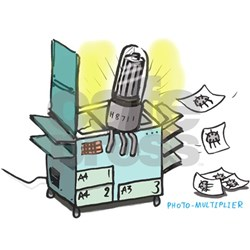
\includegraphics[scale=0.83]{fig0}
 \end{figure}

 
 \end{columns}
\framebreak

 Existe una gran variedad comercial de estos tubos sensibles a diversas longitudes de onda,
 ultravioleta, luz visible, cercana a la infrarroja y otras del espectro electromagnético.
 
 \vspace{.3cm}
 
 \textbf{Usos}:
 
 \begin{center}
   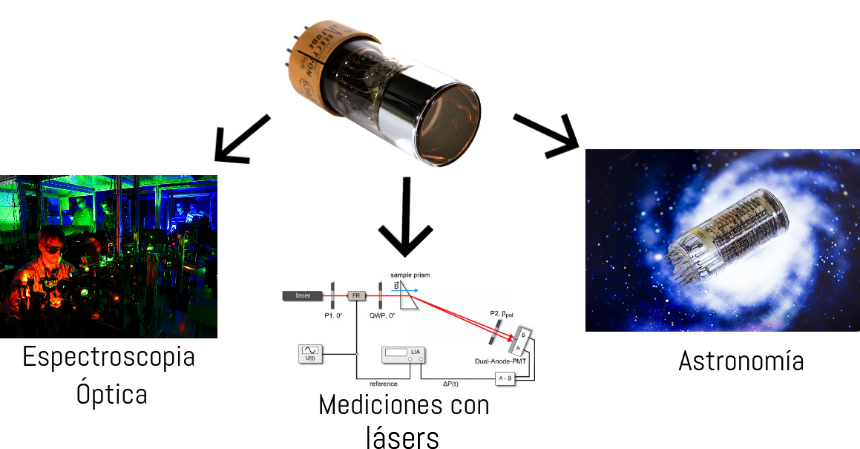
\includegraphics[scale=0.34]{fig1}
 \end{center}

 
 \end{justify}
\end{frame}

\section{Estructura simplificada de un Tubo FM}
\begin{frame}[allowframebreaks]{Estructura simplificada de un Tubo FM}
 
 \begin{columns}[c]
  \column{1.5in}
  \begin{figure}
  \center
   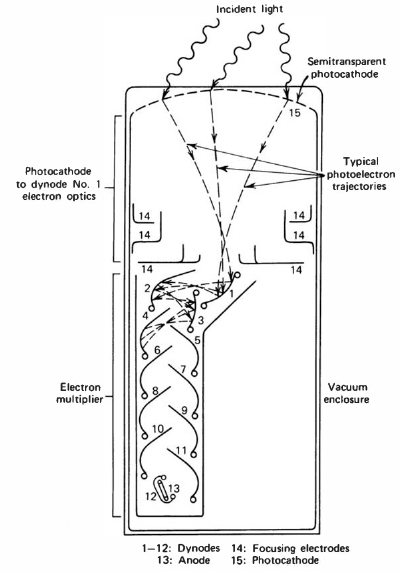
\includegraphics[scale=0.28]{fig2}
   \caption{Elementos básicos de un tubo FM}
  \end{figure}

  \column{2.5in}
  \begin{justify}
   
   \footnotesize{Una envoltura (usualmente de vidrio) sirve como una barrera de presión
   para mantener las condiciones de vacío dentro del tubo, que son requeridas
   para que los electrones de bajas energías puedan ser acelerados eficientemente
   por los campos eléctricos internos.
   
   \vspace{.3cm}
   
   Los dos mayores componentes dentro del tubo son una capa fotosensible, llamada
   el \emph{fotocátodo}, acoplado a una \emph{estructura multiplicadora de fotones}.
   El fotocátodo sirve para convertir la mayor cantidad posible de fotones de luz
   en electrones de baja energía.
   
   \vspace{.3cm}
   
   La sección de multiplicadora de electrones en un tubo FM provee una geometría
   de colección eficiente para los fotoelectrones, y sirve como un amplificador
   casi ideal para incrementar en altas cantidades su número.}
   
   
  \end{justify}

 \end{columns} 
 
 \framebreak
 
  \begin{figure}
  \center
   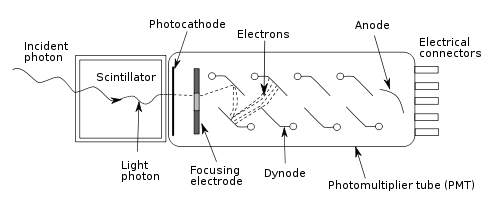
\includegraphics[scale=0.4]{fig3}
   \caption{Elementos básicos de un tubo FM}
  \end{figure}
  
  \begin{justify}
   \footnotesize{
   Luego de una amplificación a través de la estructura multiplicadora, un pulso 
   típico de centellador dará lugar a unos $10^7-10^10$ electrones, suficientes
   para servir de señal de carga para el evento original de centelleo. Esta carga
   es colectada convencionalmente en el ánodo o la etapa de salida de la estructura
   multiplicadora.
   
   \vspace{.3cm}
   
   Tubos típicos, cuando son iluminados por un pulso de luz de muy corta duración,
   producirán un pulso de electrones en un tiempo aproximado de unos pocos nanosegundos
   luego de un tiempo de espera de $20-50$ ns.}
   \end{justify}
    
\end{frame}

\section{El fotocátodo}

\begin{frame}
\begin{center}
 \Huge{\color{blue}El fotocátodo} \\
 \vspace{1cm}
 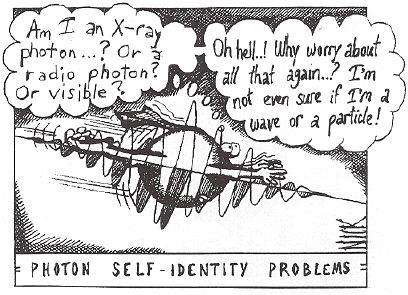
\includegraphics[scale=0.7]{fig4}
\end{center}
\end{frame}


\subsection{El proceso de fotoemisión}
\begin{frame}{El proceso de fotoemisión}
 
 \begin{justify}
  El primer paso realizado por el tubo FM es la conversión de fotones de luz incidente
  en electrones. Este proceso de foto emisión puede pensarse que ocurre en tres etapas
  secuenciales:
  
   \begin{enumerate} [<+->]
  \item La absorción de un fotón incidente y transferencia de energía a un electrón
  dentro del material fotoemisivo,
  \item la migración de ese electrón a la superficie y,
  \item el escape del electrón de la superficie del fotocátodo. 
    \begin{block}{Nota relevante}
  \footnotesize{\begin{justify}La energía que puede transferirse del fotón al electrón en el primer paso está
  dada por la energía cuántica del fotón $hv$ (típicamente $\sim 3$ eV). En el paso 2, alguna de esa energía
  se perderá por las colisiones de electrón-electrón. En el paso 3, debe haber
  la suficiente energía restante para que el electrón pase el potencial barrera
  inherente (\emph{función de trabajo.} (comúnmente $> 3$ o $4$ eV, pero para 
  metales $\sim 1.5-2$ eV)\end{justify}}
 \end{block}
 \end{enumerate}
 
 \end{justify}
  
\end{frame}

\subsection{Emisión espontánea de electrones}
\begin{frame}{Emisión espontánea de electrones}
 \begin{justify}
 La barrera de potencial superficial influencia una propiedad importante de los
 fotocátodos: \emph{el ruido termiónico}. La conducción normal de electrones
 adentro del material del fotocátodo siempre tendrá algo de energía cinética térmica
 que, a temperatura ambiente, se aproximará a los $0.025$ eV. 
 
 \vspace{.3cm}
 
 Si ese electrón está cerca de la superficie, puede escapar y dar lugar a una señal
 inducida térmica espontánea.
  
\begin{block}{Nota relevante}
 \begin{justify}
  En los metales, la tasa de emisión térmica es baja $(\sim 100 \text{m}^2\cdot \text{s})$
  debido a su potencial de barrera relativamente alto. En los semiconductores, el bajo 
  potencial de barrea lleva a tasas de emisión térmicas tan altas como $10^6-10^8 \text{m}^2\cdot \text{s}$
 \end{justify}
 \end{block}
\end{justify}
\end{frame}

\subsection{Fabricación de fotocátodos}
\begin{frame}{Fabricación de fotocátodos}
 \begin{justify}
  
  \small{Los fotocátodos pueden ser construidos tanto por capas opacas o semitransparentes.
  Un fotocátodo opaco es fabricado normalmente con un grosor un poco más grande 
  que la profundidad de escape máxima\footnotemark y es soportado por un material
  de respaldo grueso. Los fotocátodos semitransparentes generalmente no son más 
  gruesos que la profundidad de escape, son depositados en un respaldo transparente 
  (usualmente el final del vidrio del tubo FM).}
  
  \begin{block}{Nota relevante}
  \begin{justify}
   Debido a que son más fácilmente adaptables a diseños de tubo que usan una 
   ventana final plana, los fotocátodos semitransparentes son más comunes en los
   tubos FM diseñados para conteo de centelladores.
   \end{justify}
  \end{block}
  
  \begin{exampleblock}{Nota experimental}
  \begin{justify}
   Las variaciones en el espesor darán lugar a cambios correspondientes en la sensitividad 
   del fotocátodo y pueden ser una fuente de pérdida de resolución en los conteos de 
   centelladores (el problema es $\propto$ al diámetro del tubo).
   \end{justify}
  \end{exampleblock}

  \footnotetext[1]{Profundidad máxima del material, en la que los electrones puedan
  alcanzar la superficie y superar el potencial de barrera.}
  
 \end{justify}

\end{frame}

\subsection{Eficiencia cuántica y respuesta espectral}
\begin{frame}[allowframebreaks]{Eficiencia cuántica y respuesta espectral}
 \begin{justify}
  
  \small{La sensitividad de los fotocátodos se mide comúnmente en el ámbito
  de la física, y con gran significación para el conteo de centelladores
  en términos de la \emph{eficiencia cuántica (EC)} del fotocátodo.
  La eficiencia cuántica se define simplemente como}
  
  \begin{equation}
   EQ = \frac{\text{número de fotoelectrones emitidos}}{\text{número de fotones incidentes}}
  \end{equation}

  \vspace{.2cm}
  
  \small{La eficiencia cuántica sería de $100\%$ para un fotocátodo ideal. Pero
  debido a las limitaciones que les he mencionado, los fotocátodos
  comunes tienen una eficiencia cuántica máxima de $20-30\%$.}
  
  \begin{columns}[c]
    \column{2in}
  \begin{block}{Nota relevante}
  \begin{justify}
   La eficiencia cuántica de cualquier fotocátodo será fuertemente una 
   función de la longitud de onda o la energía cuántica de la luz incidente.
   \end{justify}
  \end{block}
    \column{2in}
  \begin{exampleblock}{Nota experimental}
  \begin{justify}
  Una consideración para seleccionar un fotocátodo es buscar una alta
  eficiencia cuántica sobre el rango de longitudes de onda en el 
  cual el espectro de emisión del centellador es concentrado.
   \end{justify}
  \end{exampleblock}
  \end{columns}

  \pause
  
  \begin{columns}[c]
  \column{2in}
  \begin{figure}
   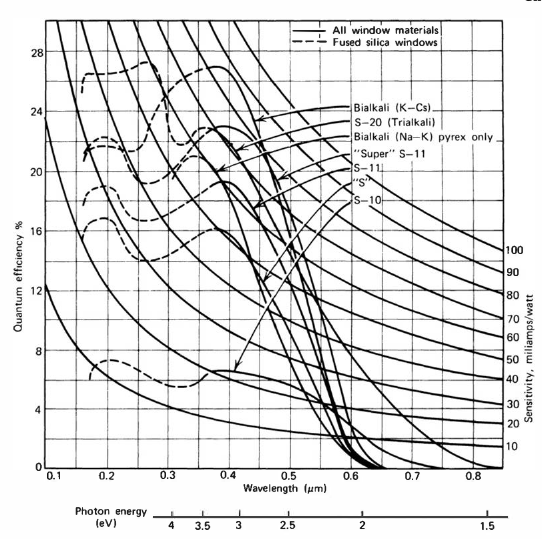
\includegraphics[scale=0.28]{fig5}
   \caption{La eficiencia cuántica es función de la longitud de onda
   o de la energía cuántica de la luz incidente}
  \end{figure}
  
  \column{2in}
  \begin{justify}
  \footnotesize{A una $\lambda$ lo suficientemente alta el electrón no tiene la suficiente
  energía para escapar la superficie del fotocátodo y la respuesta se 
  hace cero. Para vidrio normal, el límite será a $\lambda \sim 350$ nm,
  que es usualmente adecuado para la mayoría de los materiales de centelladores.}
  \end{justify}
  
  \begin{exampleblock}{Nota experimental}
   \begin{justify}
   \footnotesize{Una medida alternativa para la EQ es usada en el conteo de 
   centelladores. Debido al uso extendido de yoduro de sodio 
   activado con talio como cristal de centelleo, se habla de EQ 
   en términos de el número de fotoelectrones producidos por un
   fotocátodo dado por keV de pérdida de energía en un cristal
   de NaI(Tl) para el cual casi toda la luz es colectada.}
   \end{justify}
  \end{exampleblock}

  \end{columns}

  \framebreak
  
  \textbf{Materiales actuales para la construcción de fotocátodos}:
  
  \begin{itemize}
   \item \begin{justify}Materiales multialcalinos basados en el compuesto Na$_2$KSb,
   preparados por activación con una pequeña cantidad de cesio 
   $\Rightarrow$ EQ $\sim 30\%$.\end{justify}
   \item \begin{justify}Materiales bialcalinos basados en K$_2$CsSb activados con
   oxígeno y cesio $\Rightarrow$ $45\%$ a los 350 nm de máxima respuesta.\end{justify}
   \item \begin{justify}Materiales ultrapuros que reducen las trampas de electrones,
   reduciendo reflexiones desde el fotocátodo mediante una introducción
   de de una capa anti-reflejante entre él y la envoltura de vidrio.\end{justify}
   \item \begin{justify}Estructuras prismáticas con un alto radio de superficie 
   a volumen para aumentar la probabilidad de escape de fotoelectrones.\end{justify}
  \end{itemize}

  
 \end{justify}
\end{frame}

\section{Multiplicación de Electrones}

\begin{frame}
\begin{center}
 \Huge{\color{blue}Multiplicación de Electrones} \\
 \vspace{0.5cm}
 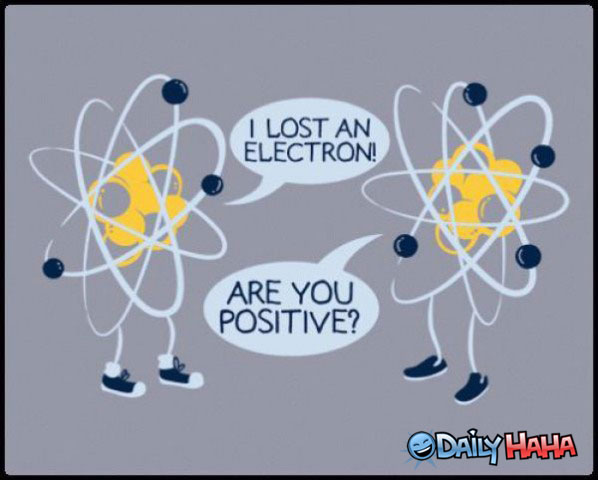
\includegraphics[scale=0.3]{fig6}
\end{center}
\end{frame}

\subsection{Emisión secundaria de electrones}
\begin{frame}{Emisión secundaria de electrones-I}


\begin{columns}[c]

 \column{2in}
\begin{figure}
   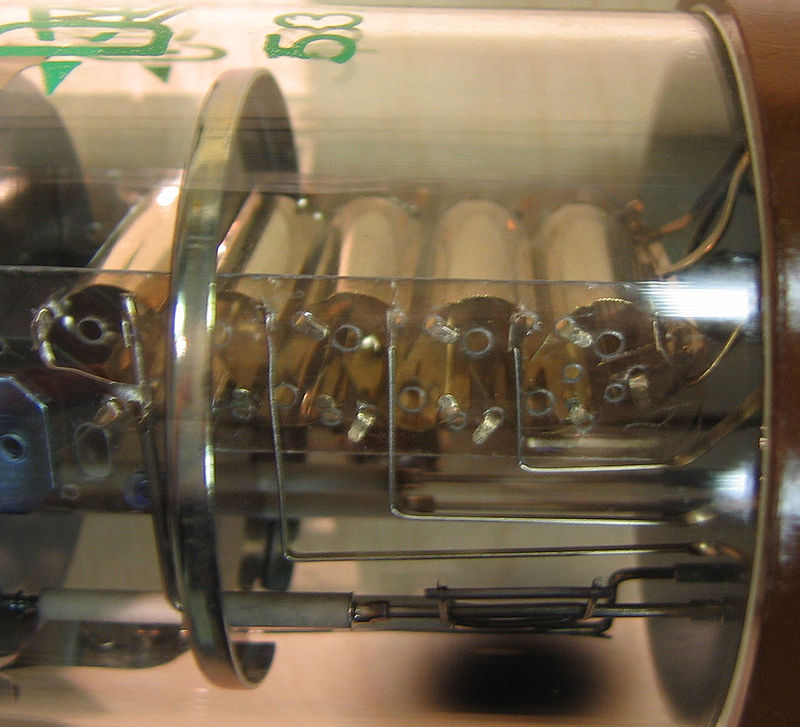
\includegraphics[scale=0.32]{fig7}
   \caption{Dos filas de dínodos dentro de un tubo FM.}
  \end{figure}
  
  \column{2.3in}
\begin{justify}
  Los electrones desde el fotocátodo son acelerados y llevados a chocar la superficie 
  de un electrodo, llamado el \emph{dínodo}. Si el material del dínodo se escoge bien,
  la energía depositada por el electrón incidente puede resultar en la re-emisión de 
  más de un electrón desde la superficie.
 \end{justify}

 \end{columns}

\begin{itemize}[<+->]

 \item[]  \begin{block}{Nota relevante}
  \begin{justify}
  \begin{footnotesize}
   El proceso de emisión secundaria de electrones es similar al proceso que acabamos 
   de ver, pero en este caso los electrones dentro del material del dínodo son 
   exitados por el paso de un electrón energético en vez de un fotón óptico.
   \end{footnotesize}
  \end{justify}
 \end{block}

\end{itemize}
\end{frame}

  
\begin{frame}{Emisión secundaria de electrones-II}

 \begin{footnotesize}Los electrones que dejan el fotocátodo tienen una energía $\sim 1$ eV, o menos. 
 Por lo tanto, si el primer dínodo tiene unos cuantos cientos de voltios positivos, 
 la energía cinética de los electrones al llegar al dínodo está determinanda por 
 el voltaje de aceleración. \end{footnotesize}
 
  \begin{exampleblock}{Nota experimental}
  \begin{footnotesize}
  \begin{itemize}[<+->]
   \item \begin{justify}
          La creación de un electrón excitado en el material del dínodo requiere una
          energía al menos igual a la del bandgap $\sim 2-3$ eV.
         \end{justify}
   \item \begin{justify}
          Es teóricamente posible que para un electrón incidente, se creen un 
          aproximado de 30 electrones exitados por cada 100 V de voltaje acelerador.
         \end{justify}
   \item \begin{justify}
          Debido a que la dirección de estos electrones es aleatoria, (1) algunos 
          no llegarán a la superficie antes de des-excitarse, (2) otros llegan 
          pero han perdido tanta energía que no pueden superar el potencial de barrera
          y no pueden escapar. Por lo que solo una pequeña fracción de electrones 
          excitados contribuirá últimamente a la emisión secundaria dada en la 
          superficie del dínodo.
         \end{justify}
   \item \begin{justify}
          La producción de electrones secundarios es una función sensible a la 
          energía de los electrones incidentes.
         \end{justify}

  \end{itemize}  
  \end{footnotesize}
 \end{exampleblock}
\end{frame}

\begin{frame}[label=milink1]{Emisión secundaria de electrones-III}

\begin{columns}[c]
    \column{2in}
 \begin{figure}
  \center
     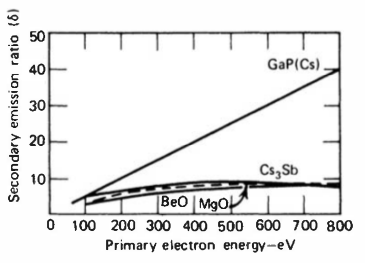
\includegraphics[scale=0.4]{fig8}
     \caption{Variación de la producción en la emisión secundaria con energía 
   de electrón primaria para algunos materias estándares de dínodos (las 
   tres de abajo) y un material NEA (negative-electron affinity) [GaP(CS)]}
   \label{fig:fig8}
   \end{figure}
   \column{2in}
 \begin{block}{Factor de multiplicación}
  El factor de multiplicación para un dínodo está dado por:
  \begin{equation*}  
   \delta=\frac{\text{\parbox{12em}{\center número de electrones secundarios emitidos}}}{\text{electrones primarios
   incidentes}}
  \end{equation*}
  \begin{justify}Este debe ser lo más grande posible para una máxima amplificación por etapa 
  en el tubo FM.
  \end{justify}
  \end{block}
  \end{columns}
\end{frame}


\subsection{Materiales de afinidad electrónica negativa}
\begin{frame}{Materiales de afinidad electrónica negativa - I}

\begin{columns}[c]

\column{2.3in}
\begin{justify}
\begin{footnotesize}
 La producción de emisión secundaria de los dínodos puede ser aumentada significativamente 
 a través del uso de materiales de \textbf{afinidad electrónica negativa} (La afinidad electrónica es la 
 variación de energía que se produce en la adición de un electrón al átomo en estado fundamenta
 y en fase gaseosa para formar el anión correspondiente. La afinidad electrónica puede ser energía desprendida,
 en cuyo caso tiene valor negativo y se trata de átomos con tendencia a captar electrones - no metales.)
 \end{footnotesize}
 \end{justify}
 \column{2in}
 
 \begin{center}
  
\includegraphics[scale=0.2]{fig9}
 \end{center}


\end{columns}
 
  \begin{block}{Nota relevante}
  El más exitoso de estos materiales ha sido el fosfuro de galio (GaP), altamente 
  dopados, a una concentración de casi $10^19$ átomos/cm$^3$ con zinc. Y una capa
  delgada de cesio.
 \end{block}

\end{frame}

\begin{frame}{Materiales de afinidad electrónica negativa - II}

\begin{figure}
 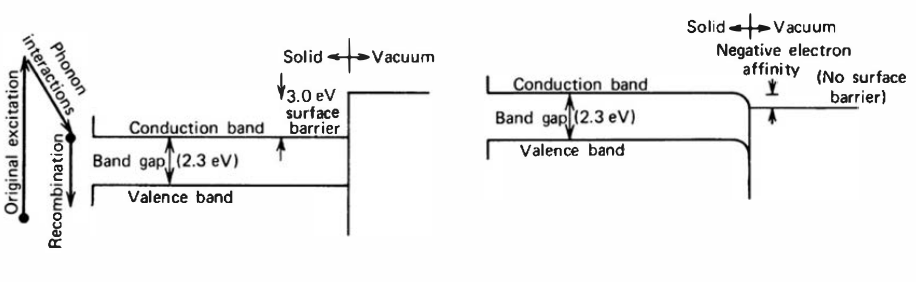
\includegraphics[scale=0.33]{fig10}
 \caption{Estructura de banda cerca de la superficie para semiconductores 
 convencionales (izquierda) y materiales NEA (derecha).}
\end{figure}

\begin{block}{Nota relevante}
\begin{justify}
 A la derecha se muestra la flexión de banda creada por el llenado de lugares 
 aceptadores en la superficie por la capa delgada de Cs. El efecto de esto, 
 es llevar el potencial de vacío más abajo que el del fondo de la banda de 
 conducción en el interior del material.
 \end{justify}
\end{block}

\end{frame}

\begin{frame}{Materiales de afinidad electrónica negativa - III}
 
 \begin{exampleblock}{Nota experimental}
  \begin{itemize}
  \item \begin{justify}
	El efecto neto es que los electrones que han llegado al fondo de la banda 
	de conducción, aún son candidatos a escapar, y se quedan así por un tiempo 100
	veces mayor que antes 
	\end{justify}
 \item \begin{justify}
        Este aumento de tiempo en que los electrones pueden escapar, aumenta 
        las probabilidades de escapa para un electrón típico\footnote{Ver figura
        5. \hyperlink{milink1}{\beamerreturnbutton{Ir}}}.
       \end{justify}
  \end{itemize}
 \end{exampleblock}
 
 \begin{block}{Nota relevante}
  Otra ventaja de utilizar materiales NEA es en tubos FM usados para 
  aplicaciones de medición temporal ultrarápida.
 \end{block}
\end{frame}

\subsection{Múltiples etapas de multiplicación}
\begin{frame}{Múltiples etapas de multiplicación - I}
 \begin{justify}
 Los electrones son guiados por otro campo eléctrico de dínodo en dínodo, en
 la cual se repite la etapa  de multiplicación varias veces. Si se requieren 
 $N$ etapas en la sección multiplicadora, la ganancia total para el tubo FM
 está dada simplemente por 
 
 \begin{equation}
  \text{Ganancia total} = \alpha \delta^N
 \end{equation}
 
 donde $\alpha$ es la fracción de todos los fotoelectrones colectados por la 
 estructura multiplicadora.
\end{justify}
 
 \begin{exampleblock}{Nota experimental}
 \begin{itemize}
 \begin{footnotesize}
\item \begin{justify}
  Los materiales de dínodo convencionales están caracterizados por valores típicos 
  de $\delta=5$ y $\alpha \sim 1$ para tubos bien diseñados. Entonces diez etapas
  resultarán en una ganancia total de $5^10$ o $10^7$. Sise utilizan materiales 
  NEA entonces $\delta \sim 55$, y la misma ganancia se puede conseguir en 4 etapas.
 \end{justify}
\item \begin{justify}
       La ganancia total de un tubo FM es una función sensible del voltaje aplicado $V$.
      \end{justify}
 \end{footnotesize}
 \end{itemize} 
 \end{exampleblock}

 
\end{frame}

\subsection{Estadística de la multiplicación de electrones}
\begin{frame}{Estadística de la multiplicación de electrones - I}

\begin{justify}
 La emisión de electrones secundarios es un proceso estadístico, y por lo tanto el 
 valor específico de $\delta$ en un dínodo dado, fluctuará de evento en evento sobre 
 su valor medio. En el modelo más simple, la producción de electrones secundarios en 
 un dínodo, puede asumirse que sigue un distribución de Poisson sobre la producción media.
 Por lo tanto para un un fotoelectrón incidente en el primer dínodo, el número de 
 secundarios productidos tiene un valor medio de $\delta$ y una desviación estándar 
 $\sigma$ de $\sqrt{\delta}$.
 \end{justify}
 
 \begin{columns}[c]

 \column{2in}
 \begin{block}{Nota relevante}
 \begin{justify}
 \begin{footnotesize}
 La varianza relativa definida por $(\sigma/\delta)^2$, es igual a $1/\delta$. Recordando 
 la distribución de Poisson, entonces es fácil ver que cuando este proceso se repite 
 sobre $N$ etapas idénticas en el tubo FM, el número medio de electrones colectados en 
 el ánodo será igual a $\delta^N$.
 \end{footnotesize}
 \end{justify}
 \end{block}
 \column{2in}
 \begin{block}{Nota relevante}
 \begin{justify}
  Si $\delta \gg 1$, entonces la varianza relativa o la expansión en la amplitud 
  del pulso de salida es dominada por fluctuaciones en la producción desde el primer
  dínodo, donde el número absoluto de electrones es el más pequeño.
  \end{justify}
 \end{block}
 \end{columns}

\end{frame}

\begin{frame}{Estadística de la multiplicación de electrones - II}
 \begin{columns}[c]
  
  \column{1.5in}
\begin{figure}
 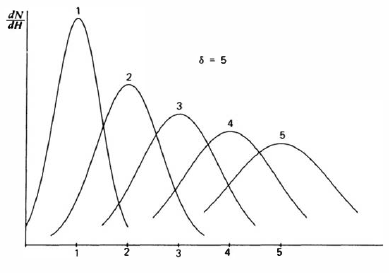
\includegraphics[scale=0.35]{fig11}
\end{figure}
  \column{1.5in}
\begin{figure}
 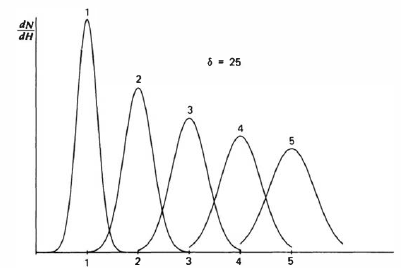
\includegraphics[scale=0.35]{fig12}
\end{figure} 
 \end{columns}
 
 \begin{exampleblock}{Nota experimental}
  \begin{justify}
  \begin{footnotesize}
   Las figuras de arriba muestran la distribución esperada en el número de 
   electrones secundarios producidos por el primer dínodo, cuando es golpeado 
   por diferentes números de fotoelectrones. Si el valor de $\delta$ es pequeño 
   es imposible separar limpiamente los eventos causados por un fotoelectrón de 
   aquellos en los que más fotoelectrones están presentes.
   \end{footnotesize}
   \end{justify}
 \end{exampleblock}
\end{frame}

\begin{frame}{Estadística de la multiplicación de electrones - III}

 \begin{columns}[c]
 
\column{2in}

\begin{figure}
 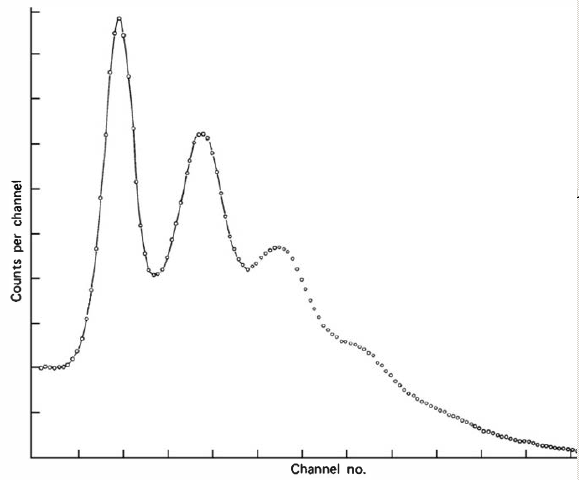
\includegraphics[scale=0.2]{fig13}
\end{figure}

\begin{exampleblock}{Nota experimental}
\begin{justify}
\begin{footnotesize}
Si los dínodos están caracterizados por valores grandes de $\delta$, la separación 
es mucho más discernible y es posible distinguir picos en la distribución correspondiente 
a números discretos de fotoelectrones hasta 4 o 5.
\end{footnotesize}
\end{justify}
\end{exampleblock}

\column{2in}

\begin{exampleblock}{Nota experimental}
\begin{justify}
\begin{footnotesize}
Algunas mediciones experimentales muestran una varianza relativa mayor que la predicha 
por el modelo de Poisson. De hecho, algunas observaciones no muestran picos, sino 
una distribución tipo exponencial. Esto ha llevado a utilizar modelos de distribución
Polya, Poisson compuestos y algunos otros. \textbf{No existe aún una descripción universal
que acomode todas las mediciones experimentales en este caso.}
\end{footnotesize}
\end{justify}
\end{exampleblock}

\end{columns}

\end{frame}

\section{Características de los tubos FM}

\begin{frame}
\begin{center}
 \Huge{\color{blue}Características de los tubos FM} \\
 \vspace{0.5cm}
 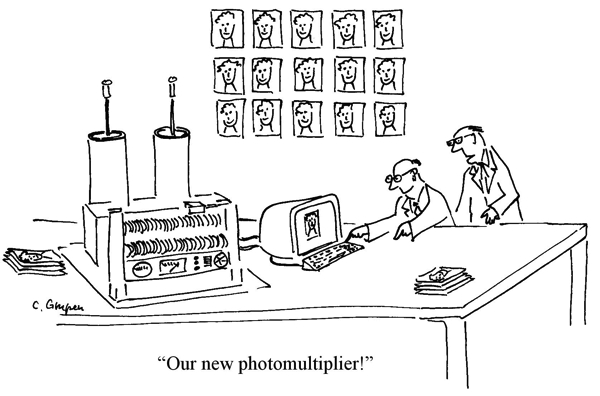
\includegraphics[scale=1]{fig14}
\end{center}
\end{frame}

\subsection{Diferencias estructurales}
\begin{frame}{Diferencias estructurales - I}
 
\begin{justify}
 Todos consisten de un fotocátodo semitransparente, una región de colección de fotoelectrones
 entre el fotocátodo y el primer dínodo, una sección de multiplicación de electrones 
 multietapa, y un ánodo para la colección de la carga amplificada. Estas estructuras están
 encerradas en una envoltura de vidrio al vacío, por la cual cables eléctricos son conducidos 
 en la base. (Les leeré un poquito sobre algunos tipos).
\end{justify}

\begin{figure}
\center
 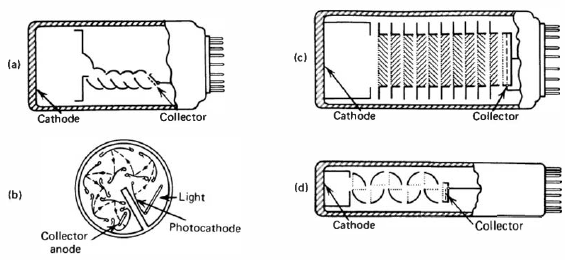
\includegraphics[scale=0.4]{fig15}
 \caption{\begin{footnotesize} Configuraciones para algunos tipos comunes de tubos FM. $(a)$ Estructura 
 lineal enfocada. $(b)$ Red circular. $(c)$ Persiana veneciana.
 $(d)$ Caja y red. \end{footnotesize}}
\end{figure}
 
\end{frame}

\begin{frame}{Diferencias estructurales - II}
\begin{columns}[c]
\column{2in}
 \begin{exampleblock}{Nota experimental}
  \begin{itemize}[<+->]
   \item \begin{justify}
          Los tubos con un plato plano de vidrio al final son los únicos tipos,
	  usados para conteo de centelladores.
         \end{justify}
   \item \begin{justify}
          Un diámetro de 5 cm es uno de las elecciones más comunes para aplicaciones 
          de centelleo.
         \end{justify}
   \item \begin{justify}
          Los tubos FM deben protegerse de vibraciones o choque mecánicos excesivos 
          para evitar un daño físico a los componentes internos.
         \end{justify}
  \end{itemize}
 \end{exampleblock}

  \column{2in}
  
  \begin{center}
 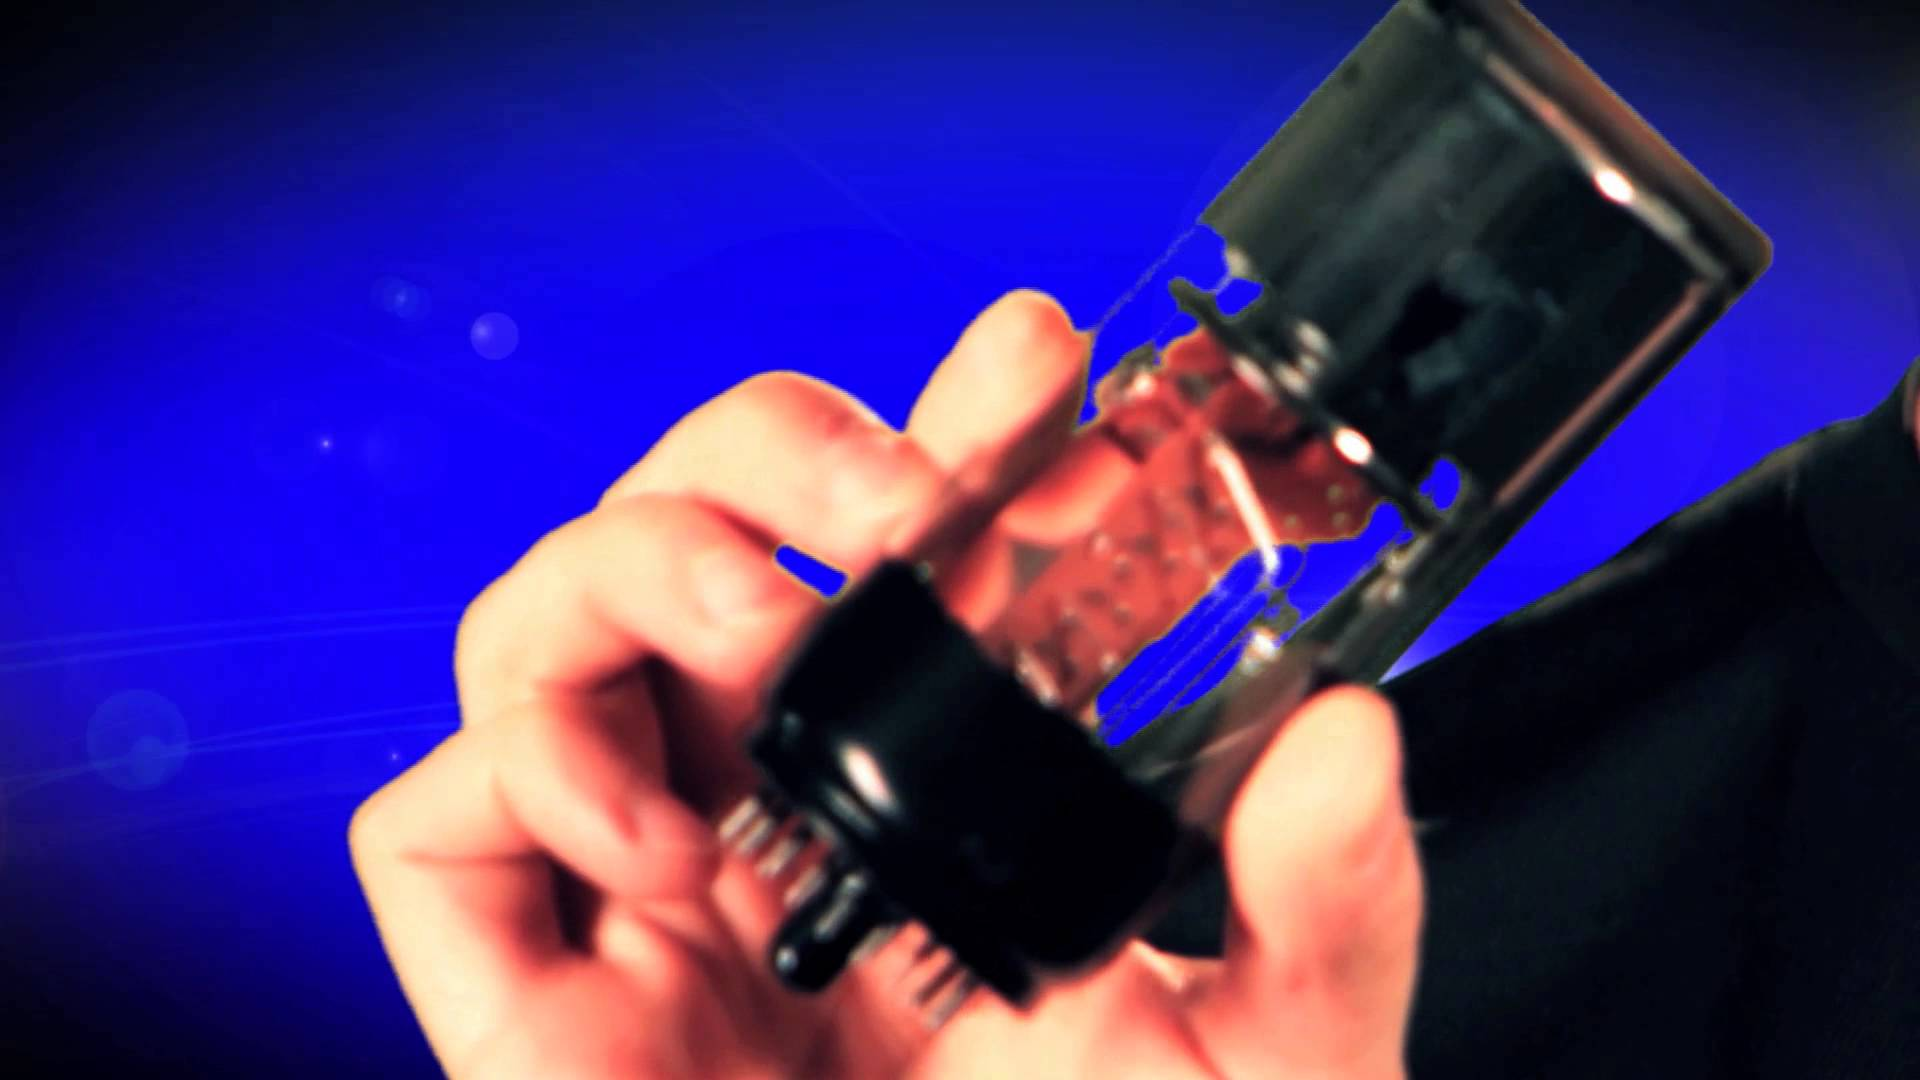
\includegraphics[scale=0.08]{fig22}
 \end{center}
  
  \end{columns}
\end{frame}

\begin{frame}{Diferencias estructurales - III}
 \begin{center}
  \Huge{\color{blue}Algunos tubos FM reales} \\
  \vspace{0.5cm}
 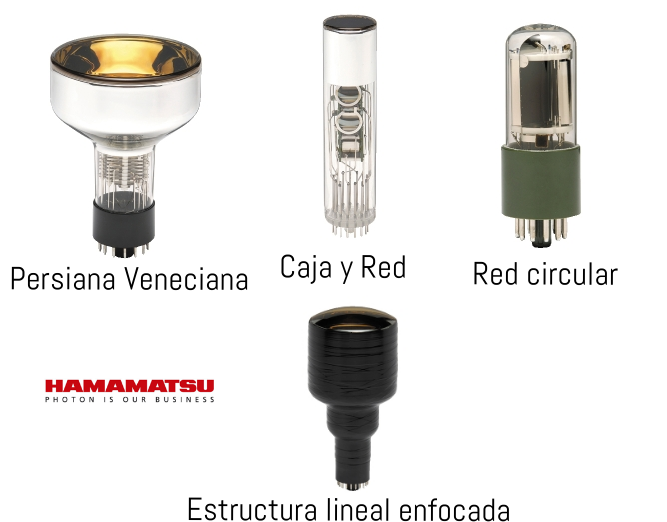
\includegraphics[scale=0.33]{fig21}
 \end{center}
\end{frame}

\subsection{Propiedades de temporización de pulsos}
\begin{frame}{Propiedades de temporización de pulsos - I}

\begin{justify}
Los tiempos característicos de un tubo FM están determinados exclusivamente 
por las trayectorias de electrones. El tiempo de tránsito de electrón de 
un tubo FM está definido por la diferencia de tiempo promedio entre la 
llegada de un fotón al fotocátodo y la colección de la subsecuente ráfaga 
de electrones en el ánodo.
\end{justify}

\begin{exampleblock}{Nota experimental}
 \begin{itemize} [<+->]
  \item \begin{justify}
         Los rangos de tiempo para el transito de electrón está entre los 
         $20-80$ ns. 
        \end{justify}
  \item \begin{justify}
         Sin embargo el tránsito solo no es de primaria importancia. El 
         esparcimiento del tiempo de tránsito es una cantidad más importante 
         porque determina la anchura de tiempo del pulso de electrones 
         que están llegando en el ánodo del tubo.
        \end{justify}
 \end{itemize}
\end{exampleblock}
 
\end{frame}

\begin{frame}{Propiedades de temporización de pulsos - II}
 
 \begin{columns}[c]
  \column{2in}
  
  \begin{figure}
  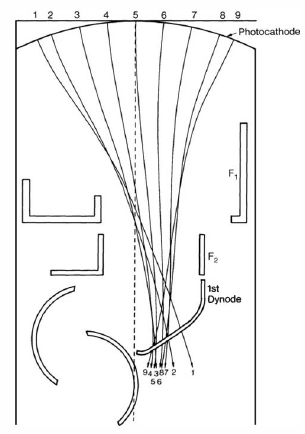
\includegraphics[scale=0.4]{fig23}
   \caption{Trayectorias generadas por computadora de los electrones 
   acelerados desde el fotocátodo al primer dínodo en un tubo FM.}
  \end{figure}
  
  \column{2.5in}
  \begin{exampleblock}{Nota experimental}
   \begin{itemize} [<+->]
    \item \begin{justify}
           La región entre el fotocátodo y el primer dínodo es crítica en 
           la determinación de las propiedades temporales. Para permitir 
           un colección uniforme sobre fotocátodos grandes, la distancia 
           entre ellos es considerablemente grande comparado con las distancias 
           entre dínodos.
          \end{justify}
    \item \begin{justify}
           La diferencia en los caminos entre un fotoelectrón que 
           deja el fotocátodo en el centro, y uno que lo deja en un 
           borde es un factor dominante en el esparcimiento observado 
           en el tiempo de tránsito.
          \end{justify}
   \end{itemize}

   
  \end{exampleblock}  
 \end{columns}

\end{frame}


\begin{frame}{Propiedades de temporización de pulsos - III}
 
 \begin{columns}[c]
  \column{2in}
  
  \begin{figure}
  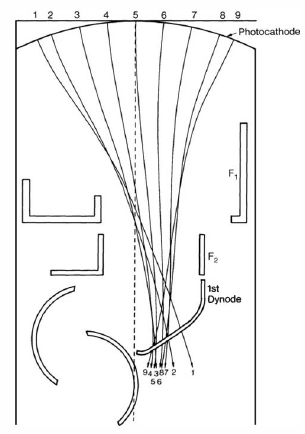
\includegraphics[scale=0.4]{fig23}
   \caption{Trayectorias generadas por computadora de los electrones 
   acelerados desde el fotocátodo al primer dínodo en un tubo FM.}
  \end{figure}
  
  \column{2.5in}
  \begin{exampleblock}{Nota experimental}
   \begin{itemize} [<+->]
    \item \begin{justify}
	  El fotocátodo usualmente es curvado para minimizar el esparcimiento 
	  del tiempo de tránsito a lo largo de su diámetro.
          \end{justify}
    \item \begin{justify}
          Una segunda fuente de esparcimiento de tiempo de tránsito surge de 
          la distribución inicial de velocidades de los fotoelectrones que 
          dejan el fotocátodo. Este efecto se puede minimizar usando una diferencia
          de voltaje más grande entre el fotocátodo y el primer dínodo.
          \end{justify}
   \end{itemize} 
  \end{exampleblock}  
 \end{columns}

\end{frame}

\begin{frame}{Propiedades de temporización de pulsos - IV}
 \begin{justify}

 Para simplificar el análisis y comparación entre diferentes fotomultiplicadores, 
 muchas de las mediciones reportadas en la literatura se concentran en el 
 esparcimiento de tiempo de tránsito debido a un sólo fotoelectrón. Por otra parte,
 si la distribución en los varios posibles esparcimientos en el tiempo de tránsito 
 se asumen gaussianos, la teoría estadística predice que el esparcimiento relativo
 en el tiempo de tránsito variará inversamente con la raíz cuadrada del número 
 de fotoelectrones.

 \end{justify}
 
 \begin{columns}[c]
  \column{2in}
  \begin{figure}
   \center 
   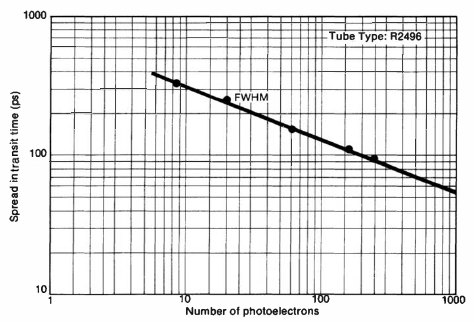
\includegraphics[scale=0.3]{fig24}
  \end{figure}
  
  \column{2in}
  \begin{block}{Nota relevante}
  \begin{justify}
   En la figura de la izquierda se verifica este comportamiento. Una alta producción 
   de luz de un centellador es importante en las aplicaciones de temporización, así 
   como en las mediciones de amplitud de pulso
   \end{justify}
  \end{block}
 \end{columns}

\end{frame}

\begin{frame}{Propiedades de temporización de pulsos - V}
\begin{exampleblock}{Nota experimental}
 \begin{justify}
 El esparcimiento temporal atribuible a la sección multiplicadora decrece con un 
 mayor voltaje entre dínodos, y el mejor desempeño en temporización normalmente es 
 obtenido operando el tubo al máximo voltaje permitido por los índices.
 
 \vspace{.3cm}
 
 Cuando se usan con centelladores inorgánicos lentas, los tubos FM son lo suficientemente
 rápidos para que su contribución al tiempo total de respuesta usualmente no sea 
 un factor importante. Sólo cuando se emplean centelladores con un tiempo de 
 decaimiento más bajo para derivar en una señal temporizadora rápida, que 
 los tubos FM se pueden convertir en un elemento significante en la determinación 
 de las propiedades de temporización resultantes.
 
 \end{justify}
\end{exampleblock}
 \end{frame}
 
\subsection{Índices máximos}
\begin{frame}{Índices máximos}

\begin{columns}[c]

\column{2in}
\begin{footnotesize}
\begin{justify}
Todos los tubos FM comerciales vienen con un conjunto de índices de voltajes máximos 
y corrientes máximas que no deben excederse durante el uso rutinario. Las especificaciones 
detalladas también darán valores individuales para los voltajes máximos entre 
el fotocátodo y el primer dínodo, dínodo a dínodo, del último dínodo al ánodo y 
del cátodo al ánodo.
\end{justify}
\end{footnotesize}

\begin{exampleblock}{Nota experimental}
\begin{justify}
 Debido a que virtualmente todos los tubos FM mostrarán un incremento en la ganancia 
 cuando el voltaje se aumenta, el valor máximo de voltaje aplicado prácticamente 
 determina la ganancia máxima que se puede obtener del tubo.
 \end{justify}
\end{exampleblock}

\column{2in}

\begin{figure}
 \center
 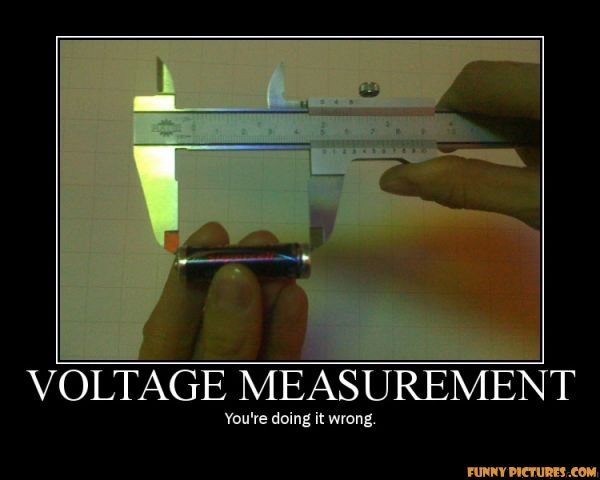
\includegraphics[scale=0.22]{fig25}
\end{figure}

\begin{figure}
 \center
 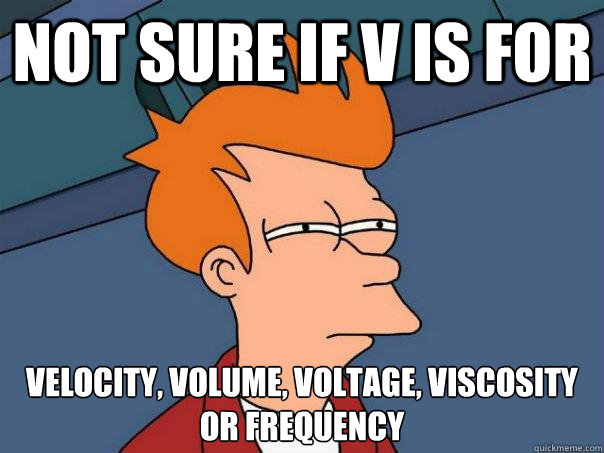
\includegraphics[scale=0.22]{fig26}
\end{figure}
\end{columns}

\end{frame}

\subsection{Especificaciones para tubos FM}
\begin{frame}{Especificaciones para tubos FM}

\begin{small}
\begin{itemize}[<+->]
 \item \begin{justify}
        \textbf{Sensitividad luminosa total (A/lm)}: Razón entre la corriente medida en el
        ánodo a un voltaje de operación y el flujo luminoso de una fuente de luz de 
        tungsteno de temperatura especificada incidente en el fotocátodo.
       \end{justify}
 \item \begin{justify}
        \textbf{Sensitividad luminosa del cátodo (A/lm)}: Definida como arriba, 
        excepto que la corriente de fotoelectrones que dejan el fotocátodo 
        es sustituida en el numerador por la corriente del ánodo.
       \end{justify}
 \item \begin{justify}
        \textbf{Sensitividad radiante total (A/W)}: Razón entre la corriente 
        del ánodo y la potencia radiante a una longitud de onda incidente dada 
        en el fotocátodo.
       \end{justify}
 \item \begin{justify}
        \textbf{Sensitividad radiante del cátodo (A/W)}: Definida como arriba, excepto 
        que la corriente del fotocátodo es sustituida por la corriente del ánodo.
       \end{justify}
 \item \begin{justify}
        \textbf{Corriente oscura}: Corriente en el ánodo medida sin la iluminación 
        del fotocátodo. 
       \end{justify}
 \item \begin{justify}
        \textbf{Tiempo de subida del pulso del ánodo}: Tiempo que toma para que el 
        pulso de salida suba de 10 a 90\% para el pico cuando el fotocátodo es 
        iluminado cuando el fotocátodo es iluminado por un flash de luz de una 
        muy poca duración.
       \end{justify}
 \item \begin{justify}
        \textbf{Ancho del pulso del ánodo}: Ancho de tiempo del pulso de salida 
        medido a la mitad de la amplitud máxima.
       \end{justify}
\end{itemize}
\end{small}
 
\end{frame}

\subsection{Linealidad}
\begin{frame}{Linealidad}
 
  \begin{justify}
  El factor de multiplicación de electrones en la mayoría de los tubos FM se mantiene 
  constante para pulsos en el rango de un solo fotoelectrón a varios miles. Bajo estas 
  condiciones la amplitud del pulso colectado en el ánodo está relacionado linealmente 
  con el número de foto electrones, y por lo tanto con la intensidad de el haz de 
  luz del centellador.
  \end{justify}
  
  \begin{block}{Nota relevante}
  \begin{justify}
   Las no-linealidades pueden surgir para pulsos muy grandes, causadas por efectos 
   de carga espacial entre el último dínodo y el ánodo, cuando el número de electrones 
   es el mayor.
   \end{justify}
  \end{block}
  
  \begin{exampleblock}{Nota experimental}
   \begin{justify}
    El voltaje de operación tal vez deba reducirse para disminuir la ganancia y prevenit 
    la distorción de la linealidad del tubo FM, aún así la amplitud de pulso integrado 
    haya incrementado solo por un factor de dos (2).
   \end{justify}
  \end{exampleblock}
 
\end{frame}

\subsection{Ruido y pulsos falsos}
\begin{frame}{Ruido y pulsos falsos - I}
 \begin{justify}
  
  Usualmente la fuente más significante de ruido aleatorio desde un tubo FM resulta 
  de los electrones termiónicos que son emitidos espontáneamente por el fotocátodo.
  Los pulsos que resultan de este proceso corresponden a un solo fotoelectrón, así que 
  su amplitud está limitada a la parte más baja en la escala.
  
 \end{justify}
 
 \begin{columns}[c]
  
 \column{2in}
 \begin{figure}
  \center 
  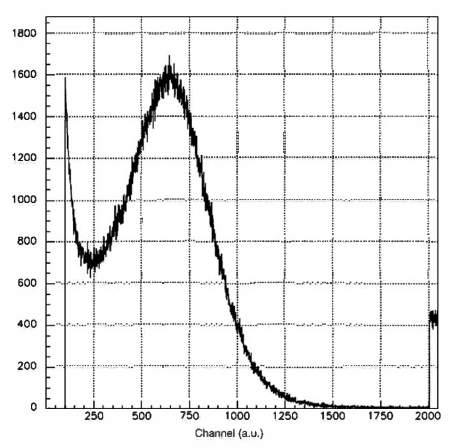
\includegraphics[scale=0.25]{fig27}
  \caption{``Espectro oscuro'' en el cual esencialmente todos los pulsos provienen de 
  electrones aislados emitidos por el fotocátodo.}
 \end{figure}

  \column{2.6in}
  \begin{exampleblock}{Nota experimental}
  \begin{itemize}[<+->]
   \item \begin{justify}
           La tasa en la que estos pulsos son observados es proporcional al área del fotocátodo,
	   y por lo tanto se deben escoger tubos con el diámetro más pequeño requerido para 
	  una aplicación en orden de minimizar estos pulsos oscuros.
         \end{justify}
  \item \begin{justify}
         Las tasas típicas de emisión espontánea a temperatura ambiente están en el 
         rango de los $10^2-10^4$ electrones/cm$^2$ $\cdot$ s. 
        \end{justify}
  \end{itemize}
  \end{exampleblock}
 
 \end{columns}
\end{frame}

\begin{frame}{Ruido y pulsos falsos - II}
 
 {\Large{\textbf{\color{red}IMPORTANTE}}}
 
 \begin{exampleblock}{Nota experimental}
    \begin{itemize}[<+->]
     \item \begin{justify}
            Para algunos fotocátodos la tasa en la cual se emiten los electrones termiónicos 
            puede ser reducida \emph{drásticamente} enfriando el tubo. Reducciones 
            por un factor de 100 pueden ser observadas con una reducción adecuada 
            de la temperatura. Para esto se puede usar hielo seco, nitrógeno líquido 
            o refrigeradores comerciales para este propósito.
           \end{justify}
     \item \begin{justify}
            Los tubos fotomultiplicadores deben guardarse en la oscuridad cuando no 
            se están utilizando. La exposición a la luz de habitación, o la solar, 
            es desastrosa cuando se está supliendo de voltaje al tubo porque altos 
            niveles de iluminación llevan a corrientes del ánodo que exceden mucho 
            los índices máximos y pueden dañar muy rápido las estructuras multiplicadoras.
           \end{justify}
     \item \begin{justify}
            No es inusual observar un incremento de hasta 100 veces o más en la tasa de 
            pulsos oscuros inmediatamente después de una exposición a luz ambiental 
            intensa.
           \end{justify}
    \end{itemize}

 \end{exampleblock}
\end{frame}

\begin{frame}{Ruido y pulsos falsos - III}
 
 \begin{justify}
 Otra fuente de pulsos oscuros se origina de la radiactividad natural en la estructura 
 del tubo. Los componentes más importantes son usualmente $^{40}$K y torio contenidos 
 en la envoltura de vidrio. Una partícula $\beta$ producida en el decaimiento radiactivo
 dará lugar a un flash de radiación Cherenkov, que puede liberar fotoelectrones del 
 fotocátodo de una manera muy parecida a los eventos de centelleo.
 \end{justify}
 
 \begin{columns}[c]
  

  \column{2in}
   \begin{figure}
    \center 
    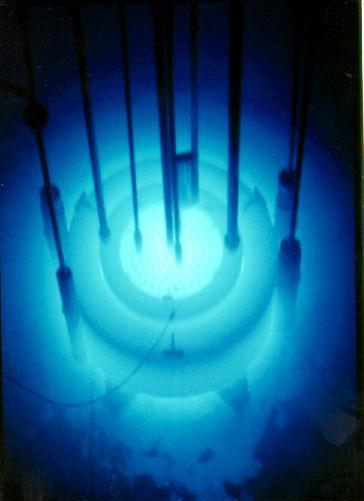
\includegraphics[scale=0.3]{fig28}
   \end{figure}

  \column{2.5in}
  \begin{block}{Nota relevante}
  \begin{justify}
  La radiación de Cherenkov es una radiación de tipo electromagnético producida
  por el paso de partículas cargadas eléctricamente en un determinado medio a 
  velocidades superiores a las de la luz en ese medio. 
  
  \vspace{.3cm}
  
  La radiación Cherenkov es un tipo de onda de choque que
  produce el brillo azulado característico de los reactores nucleares. 
  Éste es un fenómeno similar al de la generación de una onda de choque 
  cuando se supera la velocidad del sonido.
  \end{justify}
  \end{block}
  
 \end{columns}

 
\end{frame}

\begin{frame}{Ruido y pulsos falsos - IV}
 
  {\Large{\textbf{\color{blue}Radiación de Cherenkov y Rayos Cósmicos}}}

 \begin{justify} 
 
 El centelleo o luz de Cherenkov producida en el vidrio por radiación externa puede 
 ser también una fuente significativa de pulsos oscuros. Una de esas fuentes es la 
 \textbf{radiación cósmica}, que generalmente resulta en pulsos oscuros de pequeña amplitud 
 de la luz de Cherenkov producida en la ventana fina del tubo.
 
 \vspace{.3cm}
 
 Debido a la poca pérdida de energía específica de las radiaciones cósmicas 
 secundarias y la poca producción e luz en el proceso de Cherenkov, los pulsos 
 oscuros corresponden a unos pocos fotoelectrones y pueden ser descartados 
 por discriminación de amplitud en aplicaciones de centelleo típicas. Sin embargo,
  si se deben registrar eventos de poco centelleo, estos pulsos pueden ser 
  del mismo tamaño al de la señal.
  
  \begin{exampleblock}{Nota experimental}
  \begin{justify}
  La tasa de radiación cósmica puede minimizarse operando el tubo con su eje 
  mayor orientado horizontalmente, para que la ventada posterior presente la
  sección transversal mínima a los secundarios cósmicos que vienen dirigidos 
  preferencialmente en una dirección vertical.
  \end{justify} 
  \end{exampleblock}
 
\end{justify} 
\end{frame}

\subsection{Faltas de uniformidad el fotocátodo}
\begin{frame}{Faltas de uniformidad el fotocátodo}

\begin{justify}
 
 Mediciones directas han mostrado que la sensitividad de los fotocátodos, especialmente 
 los que tienen un diámetro grande, está lejos de ser uniforme a lo largo de toda el 
 área del mismo. Este problema está compuesto también por las dificultades de conseguir 
 una colección de fotoelectrones uniforme al primer dínodo desde el área del fotocátodo.
 
 \begin{exampleblock}{Nota experimental}
  \begin{itemize}[<+->]
   \item \begin{justify}
	La combinación de estos dos efectos puede llevar a situaciones en que los pulsos 
	del ánodo observados para un haz de luz dado, varíe tanto como un $30-40\%$ mientras 
	la posición de la iluminación se mueve a lo largo del área del fotocátodo.
	 \end{justify}
   \item \begin{justify}
	Estas faltas de uniformidad son un serio problema en la cuenta de centelladores
	debido q que las variaciones en la respuesta tenderán a arruinar la resolución 
	de energía del sistema. 
	 \end{justify}
  \item \begin{justify}
	\textbf{Una manera de reducir este problema es colocar un tubo de luz entre 
	el centellador y la ventana posterior del tubo FM}
	 \end{justify}
  \end{itemize}
 \end{exampleblock}

\end{justify}
\end{frame}

\subsection{Variaciones de la ganancia con la tasa de conteo}
\begin{frame}{Variaciones de la ganancia con la tasa de conteo}
 
 \begin{justify}
 Otra no-idealidad de los tubos FM de la cual el usuario debe saber, es la posibilidad 
 que la ganancia cambie durante el curso de una medición. La situación más común es 
 aquella en la que la tasa de conteo cambia por un factor grande. 
 
 \begin{exampleblock}{Nota experimental}
 \begin{itemize}[<+->]
  \item  \begin{justify}
	Las estructuras fotomultiplicadoras pueden diseñarse para minimizar estas variaciones, 
	un buen tubo no cambiará su ganancia por más de 1\% cuando la tasa de conteo cambia 
	de $10^3$ a $10^4$ por segundo.
	 \end{justify}
  \item  \begin{justify}
	 La variación gradual en la ganancia de un tubo que ocurre frecuentemente luego de 
	 un cambio grande en la corriente del tubo o la tasa de conteo se llama \emph{fatiga},
	 y puede ser un problema serio si la corriente del tubo cambia por ordenes de 
	 magnitud durante una medición.
	 \end{justify}
 \end{itemize}
 \end{exampleblock}
 
\end{justify} 
\end{frame}

\section{Equipo auxiliar requerido para los tubos FM}

\begin{frame}
\begin{center}
 {\Huge{\color{blue}Equipo auxiliar requerido para los tubos FM}} \\
 \vspace{0.5cm}
 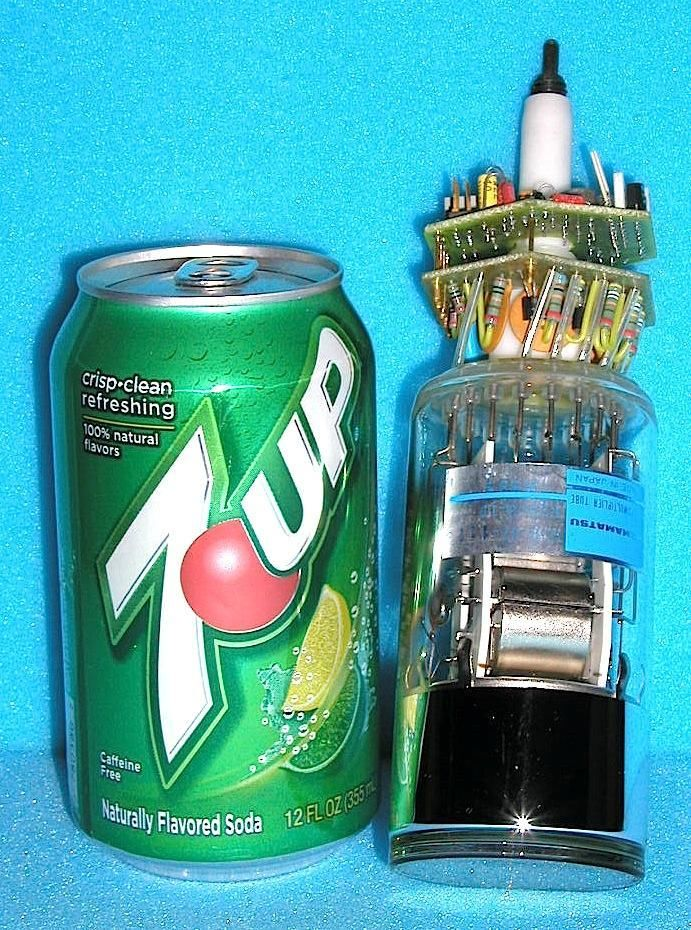
\includegraphics[scale=0.25]{fig29}
 \hspace{.3cm} \href{http://www.ebay.com/itm/HAMAMATSU-2-0-INCH-PHOTOMULTIPLIER-TUBE-/351425074352}{\color{blue}.::Link de eBay::.}
\end{center}
\end{frame}

\subsection{Alimentación de alto voltaje y divisor de voltaje}
\begin{frame}{Alimentación de alto voltaje y divisor de voltaje - I}
  
 \begin{justify} 
 Una fuente externa de voltaje debe estar conectada a los tubos FM de manera tal que 
 el fotocátodo y cada etapa multiplicadora sucesiva esté correctamente parcializada 
 con respecto a la otra.
 
 \begin{exampleblock}{Nota experimental}
 \begin{justify}
  Debido a que los electrones deben ser atraídos, el primer dínido debe estar a 
  un voltaje positivo con respecto al fotocátodo, y cada dínodo siguiente debe estar 
  a un voltaje positivo con respecto al anterior. Para una colección eficiente de 
  fotoelectrones, el voltaje entre el fotocátodo y el primer dínodo usualmente 
  es más grande que las diferencias de voltaje entre dínodos.
  \end{justify}
 \end{exampleblock}
 
\begin{exampleblock}{Nota experimental}
 \begin{justify}
  Los requerimientos de voltaje entre etapas de un tubo FM pueden, en principio, 
  ser suministrados por fuentes individuales de voltaje como baterías multi-celdas.
  Éstas son práctivas en algunas aplicaciones donde las tasas de cuentas son baja, pero 
  no son muy atractivas debido a tasas de descarga muy rápidas por la demanda 
  de corriente de etapas posteriores del tubo FM.
  \end{justify}
 \end{exampleblock}
 
 \end{justify}
\end{frame}

\begin{frame}{Alimentación de alto voltaje y divisor de voltaje - II}
 
 En la mayoría de los casos, las diferencias de voltaje son suministradas por divisores 
 de voltaje y una simple fuente de alto voltaje.
 
 \begin{figure}
  \center
  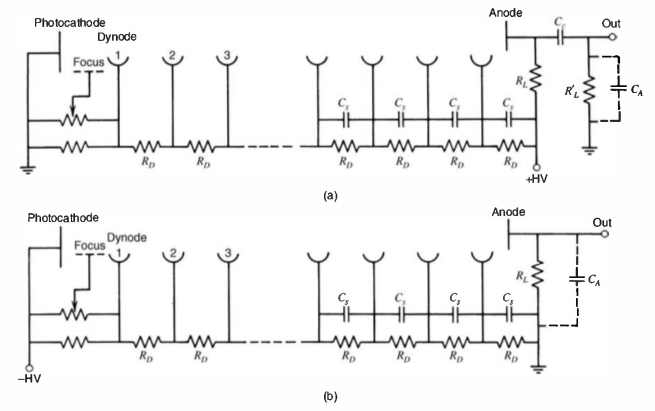
\includegraphics[scale=0.4]{fig30}
  \caption{\footnotesize Diagramas típicos de cableado para la base de un tubo FM. El esquema (a)
  utiliza alto voltaje positivo y un fotocátodo conectado a tierra. El esquema (b)
  utiliza alto voltaje negativo, y el fotocátodo debe estar aislado de la tierra. 
  Capacitancia de ánodo $C_A$, Resistencia de carga $R_L,$, Capacitores estabilizadores 
  $C_S$}
 \end{figure}
\end{frame}

\begin{frame}{Alimentación de alto voltaje y divisor de voltaje - III}
 \begin{block}{Nota relevante}
  \begin{justify}
  \footnotesize
   Si la corriente interna en el pico de un pulso se hace comparable con la corriente 
   de división, los voltajes de los dínodos normalmente comenzarán a desviarse de 
   sus valores de equilibrio, lleando a variaciones en la ganancia del tubo FM.
  \end{justify}
 \end{block}
  
  \begin{exampleblock}{Nota experimental}
  \footnotesize
   Para eliminar este efecto, es común utilizar capacitadores estabilizadores para 
   las etapas de la cuerda divisora cerca del ánodo para ayudar a mantener estos 
   voltajes posteriores del dínodo a un valor constante durante el pulso.
  \end{exampleblock}
  
  \begin{exampleblock}{Nota experimental (IMPORTANTE)}
   \footnotesize
   \begin{itemize}[<+->]
    \item \begin{justify}
          Para prevenir un cambio de voltaje entre dínodos mayor a 1\%, la carga 
          guardada en el capacitor estabilizador debe ser 100 veces más grande que 
          la emitida por ese dínodo durante el pulo
          \end{justify}
     \item \begin{justify}
          \textbf{La polaridad ($+$ o $-$) del alto voltaje usando en los tubos FM 
          es en algún sentido una elección arbitraria. Es muy importante que el usuario 
          sepa que convención ha sido utilizada por el fabricante para su tubo 
          antes del uso inicial del equipo con un tubo FM}. Aplicar la polaridad 
          errónea a un tubo FM usualmente no es fatal para el tubo, pero los 
          electrones se negarán a ``nadar cuesta arriba'' y el tubo FM no funcionará.
          \end{justify}
   \end{itemize}

  \end{exampleblock}

\end{frame}

\subsection{Recubrimiento magnético}
\begin{frame}{Recubrimiento magnético}
 
 
 \begin{columns}[c]
 
\column{2in}
 \begin{block}{Nota relevante}
  \begin{justify}
  \footnotesize
   La óptica de electrones adentro de un tubo FM es particularmente sensible a campos 
   magnéticos debido al bajo promedio de energía (del orden de los 100 eV) de los 
   electrones que viajan de etapa en etapa. Hasta la influencia del campo magnético 
   de la Tierra es suficiente para tener un efecto apreciable en la trayectoria de 
   los electrones.
  \end{justify}
  \end{block}
    
  \column{2in}
  
  
\includegraphics[scale=0.25]{fig31}

   \end{columns}
   
   
  \begin{exampleblock}{Nota experimental}
   \begin{justify}
    En las situaciones en la que es probable mover físicamente el tuvo o 
    acercarlo a equipo con campo magnético, es esencial un recubrimiento magnético 
    para prevenir cambios en la ganancia del tubo. Los más comunes consisten 
    en un cilindro fino de mu-metal (aleación de níquel-hierro y otros elementos 
    como el molibdeno) que se ajusta estrechamente a la envoltura de vidrio de 
    un tubo FM.
   \end{justify}
    \end{exampleblock}

\end{frame}

\section{Fotodiodos como sustitutos a los tubos FM}
\begin{frame}
\begin{center}
 {\Huge{\color{blue}Fotodiodos como sustitutos a los tubos FM}} \\
 \vspace{0.5cm}
 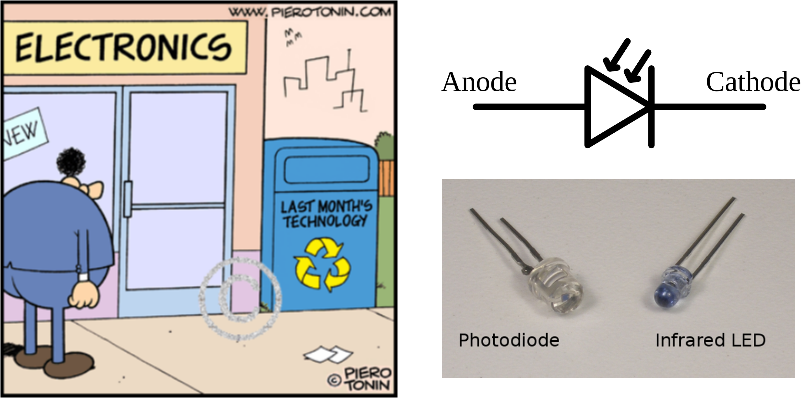
\includegraphics[scale=0.35]{fig35}
\end{center}
\end{frame}


\subsection{Potenciales ventajas}
\begin{frame}{Potenciales ventajas}
 
 \begin{justify}
  Los tubos FM son los amplificadores de luz más comúnmente usados con centelladores, t
  tanto en modo de pulso y de corriente. Sin embargo, los avances en el desarrollo de 
  fotodiodos semiconductores han llevado a la sustitución de tubos FM a dispositivos de 
  estado sólido en algunas aplicaciones.
 \end{justify}
 
 {\large{\color{blue}Algunas ventajas}:}
 
 \begin{block}{Nota relevante}
  \begin{itemize}[<+->]
   \item \begin{justify}
          Tienen una eficiencia cuántica mayor, y por lo tanto el potencial para 
          una mejor resolución energética.
         \end{justify}
  \item  \begin{justify}
          Menor consumo de potencia.
         \end{justify}
  \item  \begin{justify}
          Tamaño más compacto.
         \end{justify}
  \item  \begin{justify}
	  Mayor robustez comparado con los tubos FM usados en conteo de centelladores.
         \end{justify}
  \item  \begin{justify}
	  Son virtualmente insensibles a los campos magnéticos.
         \end{justify}
  \item  \begin{justify}
	  Su tiempo de respuesta es comparable con el de los tubos FM y también 
	  pueden ser utilizados para aplicaciones de temporización.
         \end{justify}
 
  \end{itemize}
 \end{block}
 
\end{frame}

\begin{frame}{Tipos de fotodiodos de interés}
 
 En esta introducción que haremos sobre los fotodiodos, nos enfocaremos en tres 
 diseños que son los que han recibido más atención como posibles sustitutos a los 
 tubos FM.
 
 \begin{columns}[c]
  
  \column{3in}
 
 \begin{itemize}
  \item \begin{justify}
         \textbf{Fotodiodos convencionales}: También llamados fotodiodos PIN; no 
         tienen ganancia interna y operan convirtiendo directamente los fotones 
         ópticos desde el detector de centelleo a pares de electrón-hoyo que 
         son colectados simplemente.
        \end{justify}
  \item \begin{justify}
         \textbf{Fotodiodos de avalancha}: Incorporan la ganancia interna a través 
         del uso de campos eléctricos fuertes que incrementan el número de 
         portadores de carga que son colectados.
        \end{justify}
  \item \begin{justify}
         \textbf{Fotomultiplicadores de silicio}: Son arreglos de muchos fotodiodos 
         de avalancha operados en modo Geiger.
        \end{justify}
 \end{itemize}
 
 \column{2in}
  \center
  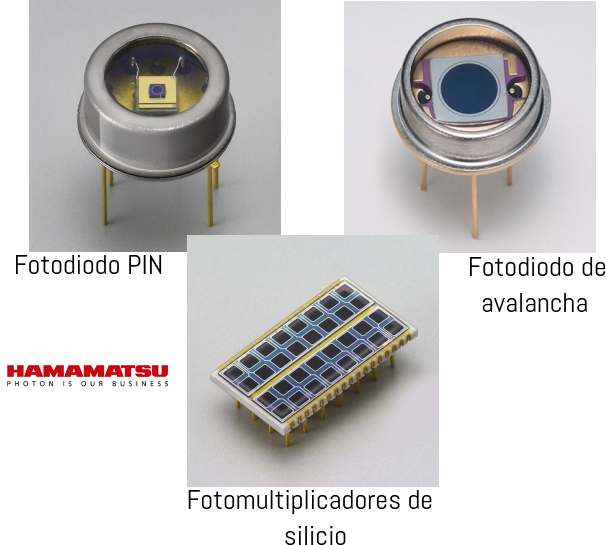
\includegraphics[scale=0.2]{fig39}
  
  \end{columns}
 
\end{frame}

\subsection{Fotodiodos convencionales}

\begin{frame}{Fotodiodos convencionales - I}

\begin{justify}
La luz incide en una ventana de entrada, hecha de semiconductor (SM) tipo $p$\footnote{Este 
tipo de SM se obtiene llevando a cabo un proceso de dopado, añadiendo un 
cierto tipo de átomos al SM para aumentar el número de portadores de cargas libres, 
en este caso positivos o huecos.}, que se mantiene lo más delgada posible para mejorar 
la transmisión de luz al volumen activo de silicio. Los electrones y hoyos producidos 
por la luz son colectados en las fronteras de la región-$i$ central, llevados por 
el campo eléctrico resultante del voltaje aplicado. La carga inducida correspondiente 
es procesada en un pre-amplificador para producir una pulso de señal de salida.
\end{justify}

\begin{figure}
 \center 
 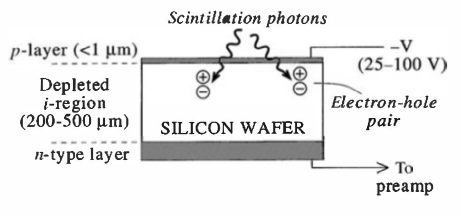
\includegraphics[scale=0.42]{fig40}
 \caption{Configuración básica de un fotodiodo convencional}
\end{figure}

\end{frame}

\begin{frame}{Fotodiodos convencionales - II}
 
 \begin{exampleblock}{Nota experimental}
  
  \begin{itemize}
   \item \begin{justify}
          Debido a la baja amplitud de la señal, el ruido electrónico es un problema 
          muy importante en el modo de operación de pulsos, especialmente para detectores 
          de gran área y radiaciones de baja energía.
         \end{justify}
    \item \begin{justify}
          Sakai midió que la resolución energética a unos 662 keV puede ser hasta 2 veces menor que 
          las mediciones en un tubo FM. Las diferencias son mucho menores para rayos 
          gamma de alta energía, pero el rendimiento de los tubo FM siempre era mejor.
         \end{justify}
  \end{itemize}  
 \end{exampleblock}

 \begin{block}{Nota relevante}
 \begin{itemize}
  \item \begin{justify}
          Aplicaciones exitosas hoy en día se limitan a radiaciones de alta energía 
          y diodos de diámetros pequeños, para los cuales la corriente oscura asociada 
          y capacitancia son pequeñas.
         \end{justify}
 \item  \begin{justify}
          Los fotodiodos convencionales se han convertido en el detector de luz
          por excelencia para centelladores en modo corriente usadas en tomografías 
          computacionales de rayos-X, y escáneres para imágenes médicas.
         \end{justify}
 \end{itemize}
 \end{block}
\end{frame}

\begin{frame}{Fotodiodos convencionales - III}
 
 El ruido en estos foto diodos surge principalmente de dos fuentes distintas:
 
 \begin{enumerate}
  \item \begin{justify}
	  \textbf{Ruido en serie}: Se origina en la etapas iniciales de 
	  preamplificación. Aumentan con la capacitancia del detector.
	\end{justify}
  \item \begin{justify}
         \textbf{Ruido paralelo}: Se origina debido a grandes fluctuaciones en 
         la corriente de fuga en el fotodiodo. Aumenta con el tamaño del fotodiodo.
        \end{justify}
 \end{enumerate}
 
 \begin{exampleblock}{Nota experimental}
  \begin{itemize}[<+->]
   \item \begin{justify}
          La capacitancia del fotodiodo decrecerá mientras su grosor aumenta, pero 
          la coriente de fuga tenderá a aumentar.
         \end{justify}
   \item \begin{justify}
          Los fotodiodos comunes para aplicaciones de centelladores se fabrican usando 
          ``obleas'' de silicio entre los $300-500$ $\mu$m.
         \end{justify}
   \item \begin{justify}
          Para los fotodiodos típicos, fabricados con silicio, los niveles de ruido 
          son mucho mayores que en los tubos FM equivalentes.
         \end{justify}      
   \item \begin{justify}
          El rápido aumento en la corriente oscura (que es una fuente de ruido) 
          a temperatura ambiente, hace que no se usen mucho los fotodiodos de silicio
          en aplicaciones que requieren altas temperaturas. Fotodiodos exitosos 
          que permiten reducir este efecto están hechos de cristales de yoduro de 
          mercurio.
         \end{justify}
  \end{itemize}

 \end{exampleblock}

\end{frame}

\subsection{Fotodiodos de avalancha}
\begin{frame}{Fotodiodos de avalancha - I}
 \begin{justify}
 La pequeña carga producida en un fotodiodo convencional por un evento de centelleo 
 típico, puede aumentarse a través de un proceso de avalancha que ocurre en un 
 semiconductora altos valores del voltaje aplicado. Los portadores de carga se 
 aceleran lo suficiente entre colisiones para crear pares de electrón-hoyo adicionales 
 a lo largo del camino de colección. 
 \end{justify}
 
 \begin{exampleblock}{Nota experimental}
  \begin{itemize}
   \item \begin{justify}
          La ganancia interna ayuda a aumentar la señal más allá del nivel de 
          ruido electrónico y permite una buena resolución energética en modo 
          de pulso a más bajas energías de radiación que las posibles con 
          fotodiodos convencionales.
         \end{justify}
    \item \begin{justify}
         Debido a que el factor de ganancia es muy sensible a la temperatura y 
         al voltaje aplicado, éstos requieren suplidores bien regulados de 
         alto voltaje para una operación estable.
         \end{justify}
     \item \begin{justify}
         La dependencia de la ganancia con la temperatura es fuerte comparada con 
         los tubos FM, ésta puede decrecer hasta 2\% por cada $^\circ$C aumentado.
         \end{justify}
  \end{itemize}

 \end{exampleblock}
 
\end{frame}

\begin{frame}{Fotodiodos de avalancha - II}
\begin{justify}
\footnotesize
 Uno de los fotodiodos de avalancha más comunes se conocen como los de configuración 
 ``reach-through''. La luz entra por la capa fina $p^+$ de la izquierda del diagrama, 
 e interactúa en la región $\pi$ que constituye la mayoría del grosor del diodo. Los 
 resultados de la interacción son pares electrón-hoyo, y el electrón es llevado 
 a la derecha a través de la porción de deriva y a la región multiplicadora donde 
 existe un alto campo magnético. Aquí se crean pares electrón-hoyo adicionales, aumentando 
 la señal medida.
\end{justify} 
 
\begin{columns}[c]
 
 \column{2in}
 \begin{figure}
  \center 
  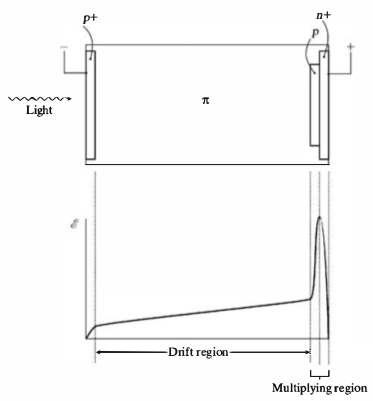
\includegraphics[scale=0.33]{fig41}
 \end{figure}

 \column{2.5in}
 
 \begin{exampleblock}{Nota experimental}
 \footnotesize
  \begin{itemize}
   \item \begin{justify}
          Son comunes factores de ganancia de unos cuantos cientos, bajo circunstancias 
          normales.
         \end{justify}
    \item \begin{justify}
          Este aumento de la señal es suficiente para permitir medir niveles muchos 
          más bajos de luz, o medir energías más baja en su uso con centelladores.
         \end{justify}
    \item \begin{justify}
          Pueden conseguirse eficiencias cuánticas tan altas como el 80\% en los 
          picos de la longitud de onda, con recubrimientos antirelfectivos, típicamente
          en el rango de los $500-600$ nm\footnote{Leer unas notas del libro p. 330}.
        \end{justify}
  \end{itemize}

 \end{exampleblock}

 
\end{columns}
\end{frame}

\subsection{Fotomultiplicadores de silicio}
\begin{frame}{Fotomultiplicadores de silicio - I}

\begin{block}{Nota relevante}
 \begin{justify}
  \textbf{Modo Geiger}: Justo como en los detectores de gas, se llega a un punto en 
  si el voltaje se aumenta lo suficiente donde el proceso de avalancha ``escapa''. Mientras 
  nos acercamos a este valor del voltaje, las regiones de multiplicación de varios 
  fotoelectrones comienzan a unirse en una sola avalancha. Entonces decimos que el 
  diodo entra en modo ``Geiger'' en el cual la carga producida en la interacción inicial 
  de fotones, es en principio, multiplicada sin límite.
 \end{justify}
\end{block}

\begin{exampleblock}{Nota experimental}
 \begin{itemize}
  \item \begin{justify}
         Los fotodiodos de avalancha en modo Geiger pueden producir un gran pulso de 
         salida de tan solo un fotón incidente.
        \end{justify}
  \item \begin{justify}
         Fotodiodos de avalancha de un solo fotón (SPAD) han sido desarrollados y mejorados 
         las últimas décadas, y están siendo aplicados en telecomunicaciones, mediciones 
         de tiempo de vida con fluorescencia y mediciones con láser. 
        \end{justify}


 \end{itemize}

\end{exampleblock}
\end{frame}


\begin{frame}{Fotomultiplicadores de silicio - II}
 
 {\large{\color{blue}Arreglos de fotodiodos de avalancha en modo Geiger}}
 
 \begin{justify}
 \small
  Para aplicaciones normales de centelladores en las cuales una amplificación proporcional 
  al número original de pares de electrones-hoyos es requerida, el modo Geiger de una 
  sola celda es de poco interés, debido a que toda la información de este número 
  original es perdida. Por lo tanto se han desarrollado arreglos de muchos fotodiodos 
  de avalancha en modo Geiger de pequeñas dimensiones que solucionan este problema, 
  los cuales son conocidos como fotomultiplicadores de silicio (SiPM).
 \end{justify}
 
 \begin{block}{Nota relevante}
  \begin{itemize}[<+->]
   \item \begin{justify}
          Los fotomultiplicadores de silicio son arreglos de pequeñas celdas de 
          fotodiodos de avalancha, cada una con dimensiones de decenas de micrones, 
          producidos usando procesos CMOS en un chip de silicio.
         \end{justify}
   \item \begin{justify}
          El número de celdas que producen una avalancha es proporcional al número de 
          fotones incidentes en el proceso de centelleo.
         \end{justify}
   \item \begin{justify}
          Debido a que los detectores de centelleo producen varios miles de fotones 
          de luz en su ventana de salida, el número de celdas debe ser un múltiplo 
          grande del número de fotones colectado para poder hacer esto. Son comunes 
          los arreglos de $10^4$ celdas o más por lo mismo.
         \end{justify}
  \end{itemize}

 \end{block}

\end{frame}

\begin{frame}{Fotomultiplicadores de silicio - III}
 
 {\large{\color{blue}Pulsos oscuros y ruido}}
 
 \begin{justify}
  Debido a que los fotodiodos de avalancha den modo Geiger son muy sensible a 
  un solo fotoelectrón, también lo son a electrones generados térmicamente en la 
  banda de conducción. Estos electrones llevan a eventos térmicos falsos que 
  agregan una componente de ruido aleatorio a la señal de centelleo.
 \end{justify}
 
 \begin{columns}[c]
 
 \column{2in}
 \begin{exampleblock}{Nota experimental}
 \small
  \begin{itemize}
   \item \begin{justify}
          La tasa ``oscura'' observada en un SiPM puede ser tan grande como $10^6$
          pulsos/s por mm$^2$ a temperatura ambiente.
         \end{justify}
         \item \begin{justify}
         La mayoría de estos eventos corresponden al disparo de una sola celda. Por 
         lo que si la medición consiste en buscar pulsos desde solo un fotón, la 
         tasa oscura espontánea puede ser muy alta.
         \end{justify}
  \end{itemize}
  
 \end{exampleblock}
 
 \column{2.3in}
  \begin{figure}
   \center
   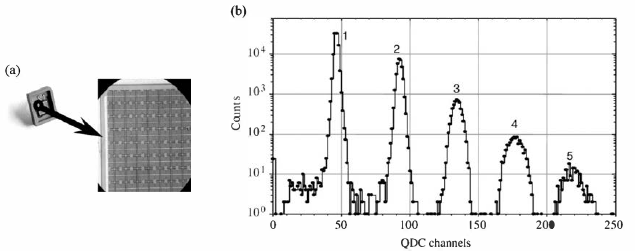
\includegraphics[scale=0.27]{fig42}
  \end{figure} 
  
  
  \end{columns}
\end{frame}

\section{Análisis de la forma de los pulsos de centelladores}
\begin{frame}
\begin{center}
 {\Huge{\color{blue}Análisis de la forma de los pulsos de centelladores}} \\
 \vspace{0.5cm}
 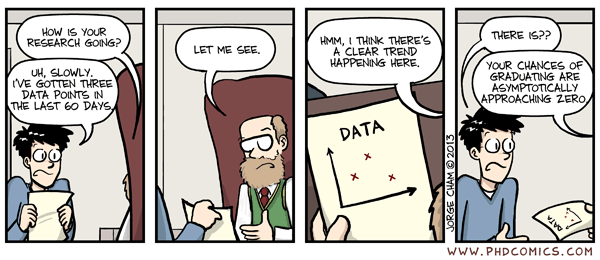
\includegraphics[scale=0.5]{fig43}
\end{center}
\end{frame}

\begin{frame}{Análisis de la forma de los pulsos de centelladores - I}
 
 \begin{block}{Nota relevante}
  \begin{itemize}[<+->]
   \item \begin{justify}
          La forma del pulso de voltaje producido en el ánodo de un tubo FM luego de 
          un evento de centelleo depende de la constante de tiempo del circuito del 
          ánodo.
         \end{justify}
  \item \begin{justify}
         Podemos identificar dos extremos los cuales son los más comúnmente usados 
         con el conteo de centelleos. El primero corresponde a situaciones en la 
         cual la constante de tiempo es seleccionada de manera tal que es \textbf{grande} 
         comparada con el tiempo de decaimiento del centellador. El otro extremo 
         se obtiene ajustando la constante de tiempo para que sea mucho \textbf{menor} 
         que el tiempo de decaimiento del centellador.
        \end{justify}

  \end{itemize}

 \end{block}
\end{frame}

\begin{frame}{Análisis de la forma de los pulsos de centelladores - II}
 
 El circuito del ánodo puede ser idealizado como en la figura de abajo.
 
 \begin{columns}[c]

\column{2in}
 \begin{figure}
  \center 
  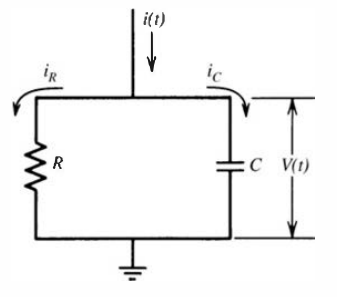
\includegraphics[scale=0.5]{fig44}
 \end{figure}
 
 \column{2in}
 
 \begin{justify}
  $C$ representa la capacitancia del ánodo, más la capacitancia del cable conector 
  y la capacitancia de entrada del circuito al cual el ánodo está conectado. La 
  resistencia de carga $R$ puede ser una resistencia física conectada a 
  la basa del tubo, o, a la impedancia del circuito conectado. La corriente que 
  fluye por el ánodo $i(t)$ es simplemente la corriente de electrones de un pulso 
  simple, supuesto a comenzar en $t=0$.
 \end{justify}
 \end{columns}
\end{frame}

\begin{frame}{Análisis de la forma de los pulsos de centelladores - III}
 
 \begin{justify}
 La forma de $i(t)$ influenciará la forma del pulso de voltaje del ánodo, y para 
 el análisis breve que haremos, utilizaremos una representación simplificada 
 de un pulso de electrones típico luego de un evento de centelleo. La componente 
 principal de la luz emitida en la mayoría de los centelladores puede ser 
 representada como un simple decaimiento exponencial.
 
 \vspace{.3cm}
 
 Si el esparcimiento del tiempo de tránsito del tubo FM es pequeño comparado con 
 este tiempo de decaimiento, entonces un modelo realista de la corriente de electrones 
 que llega al ánodo del tubo FM es simplemente
 
 \begin{equation}
  i(t) = i_0e^{-\lambda t},
 \end{equation}
 
 donde $\lambda$ es la constante de decaimiento del centellador. La corriente 
 inicial $i_0$puede representarse en términos de la carga total $Q$ colectada 
 sobre el pulso entero como $i_0 = \lambda Q$, por lo tanto
 
 \begin{equation}
  i(t) = \lambda Q e^{-\lambda t}
 \end{equation}
 \end{justify}
 
\end{frame}

\begin{frame}{Análisis de la forma de los pulsos de centelladores - IV}
 
 \begin{justify}
 Para derivar el pulso de voltaje $V(t)$ esperado en el ánodo, notamos que la 
 corriente que fluye al circuito paralelo $RC$ debe ser la suma de la corriente 
 que fluye a la capacitancia $i_C$ y la corriente sobre la resistencia $i_R$, 
 $i(t) = i_C + i_R$. Luego de unas sustituciones y trabajando sobre las anteriores 
 ecuaciones llegamos a una ecuación diferencial de primer orden no homogénea con 
 condición inicial $V(0) = 0$, cuya solución es 
 
 \begin{equation}
  V(t) = \frac{1}{\lambda - \theta}\frac{\lambda Q}{C}(e^{-\theta t} - e^{- \lambda t}),
 \end{equation}

 donde $\theta \equiv 1/(RC)$ es el recíproco la constante de tiempo del ánodo.
 
 \end{justify}
\end{frame}

\subsection{Caso 1. Constante de tiempo grande}

\begin{frame}{Constante de tiempo grande - I}
 
 Si la constante de tiempo se hace grande comparada con el tiempo de de decaimiento del 
 centellador, entonces $\theta << \lambda$, y tenemos entonces que 
 
 \begin{equation}
  V(t) \cong \frac{Q}{C}(e^{-\theta t} - e^{-\lambda} t)
 \end{equation}
 
 Debajo se muestra este pulso graficado. 

 \begin{columns}[c]
 
 \column{2in}
 
 \begin{figure}
  \center
  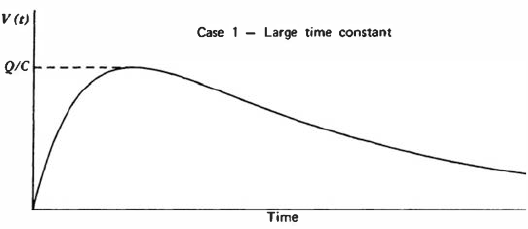
\includegraphics[scale=0.3]{fig45}
  \end{figure}

 
 \column{2in}
  El comportamiento a valores pequeños de $t$ es ahora
  
  \begin{equation*}
   V(t) = \frac{Q}{C}(1 - e^{-\lambda t}), \quad \left(t \ll \frac{1}{\theta} \right)
  \end{equation*}
  
  y para $t$ grande 
  
  \begin{equation*}
   V(t) = \frac{Q}{C}e^{-\theta t}, \quad \left(t \gg \frac{1}{\lambda} \right)
  \end{equation*}
 
 \end{columns}

\end{frame}

\begin{frame}{Constante de tiempo grande - II}
 
 Las siguientes observaciones importantes pueden hacerse,
 
 \begin{block}{Nota relevante}
  \begin{itemize}[<+->]
   \item \begin{justify}
          La parte principal del pulso tiene un comportamiento temporal $(1-e^{-\lambda t})$ 
          y su tiempo de subida es determinado por la la constante de decaimiento del
	  centellador $\lambda$. Los centelladores rápidos tienen valores grandes 
	  de $\lambda$ que llevan a pulsos que suben rápidamente.
         \end{justify}
   \item \begin{justify}
          La cola del pulso tiene un comportamiento temporal $e^{-\theta t}$ y por 
          lo tanto decae a una tasa determinada por la constante temporal del 
          circuito del ánodo $RC \equiv 1/\theta$.
         \end{justify}
     \item \begin{justify}
          La amplitud del pulso está dada simplemente por $Q/C$, pero este valor 
          es alcanzado solo si $\theta \ll \lambda$. Es decir, como hemos establecido, 
          la constante de tiempo del circuito debe ser más grande que el tiempo de 
          decaimiento del centellador.
         \end{justify}      
  \end{itemize}
 \end{block}
\end{frame}

\begin{frame}{Constante de tiempo grande - III}
 
 \begin{exampleblock}{Nota experimental}
  \begin{itemize}[<+->]
   \item \begin{justify}
          La mayoría de la cuenta de centelladores se hace en este modo debido a 
          que la altura del pulso es maximizada y las fuentes subsecuentes de ruido 
          tendrán un efecto degradante mínimo en la resolución de altura del pulso.
          \end{justify}
   \item \begin{justify}
	  La amplitud del pulso conseguida no es sensible a cambios en la resistencia 
	  de carga o a cambios pequeños en los tiempos característicos del pulso 
	  de electrones.
         \end{justify}
   \item \begin{justify}
          El usuario debe escoger una constante de tiempo al menos unas $5-10$ veces 
          más grande que el tiempo de decaimiento del centellador pero que no sea
          excesivamente grande para prevenir un apilado innecesario de la cola de 
          un pulso precedente. 
         \end{justify}      
  \end{itemize}
 \end{exampleblock}
\end{frame}

\subsection{Caso 2. Constante de tiempo pequeña}

\begin{frame}{Constante de tiempo pequeña - I}
En el extremo opuesto, la constante de tiempo del ánodo se hace pequeña comparada 
con el tiempo de decaimiento del centellador, o $\theta >> \lambda$, entonces 

\begin{equation}
 V(t) \approx \frac{\lambda}{\theta}\frac{Q}{C}(e^{-\lambda t} - e^{-\theta t})
\end{equation}

Debajo se muestra este pulso graficado. 

  \begin{columns}[c]
  
 \column{2in}
 
\begin{figure}
  \center
  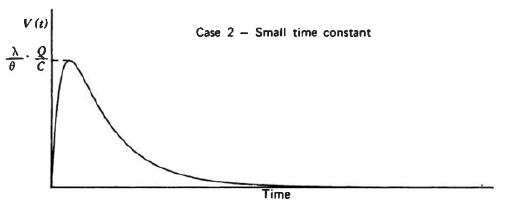
\includegraphics[scale=0.37]{fig46}
  \end{figure}


 \column{2in}
  El comportamiento a valores pequeños de $t$ es ahora
  
  \begin{equation*}
   V(t) = \frac{\lambda}{\theta}\frac{Q}{C}(1 - e^{-\theta t}), \quad \left(t \ll \frac{1}{\lambda} \right)
  \end{equation*}
  
  y para $t$ grande 
  
  \begin{equation*}
   V(t) = \frac{\lambda}{\theta}\frac{Q}{C}e^{-\lambda t}, \quad \left(t \gg \frac{1}{\theta} \right)
  \end{equation*}
 
 \end{columns}
\end{frame}

\begin{frame}{Constante de tiempo pequeña - II}
 
 Las siguientes conclusiones generales ahora aplican,
 
 \begin{block}{Nota relevante}
  \begin{itemize}[<+->]
   \item \begin{justify}
          La parte principal del pulso tiene un comportamiento temporal $(1 - e^{-\theta t})$, 
          que está determinado por la constante de tiempo del ánodo $RC \equiv 1\theta$.
         \end{justify}
   \item \begin{justify}
          La cola del pulso tiene comportamiento temporal $e^{-\lambda t}$, el cual 
          es idéntico al de la luz de centelleo.
         \end{justify}
     \item \begin{justify}
          La amplitud máxima del pulso es ahora $(\lambda Q/\theta C)$, mucho más 
          pequeña que en el caso 1, en el cual el máximo era $(Q/C)$, porque por 
          definición para el caso 2 $\lambda \ll \theta$.
         \end{justify}      
  \end{itemize}
 \end{block}
\end{frame}

\begin{frame}{Consideraciones un poco más realistas}

\begin{justify}
\small
El modelo simplificado que hemos usado asume una corriente $i(t)$ continua y suave, 
no representa la naturaleza ``agrupada'' de la corriente que surge últimamente 
del ánodo de fotoelectrones discretos. En el caso 1, los efectos de discreción 
son muy suavizados por el proceso de integración de corrientes que se hace. En el 
caso 2, no se hace ninguna integración y el pulso es mucho más sensible a fluctuaciones 
que se originan de la naturaleza estadística de la producción de fotoelectrones. Estas 
fluctuaciones en la forma del pulso y la amplitud son muy significantes para los eventos 
de centelleo débiles, que producen solo un pequeño número de fotoelectrones.
\end{justify}

\begin{figure}
 \center
 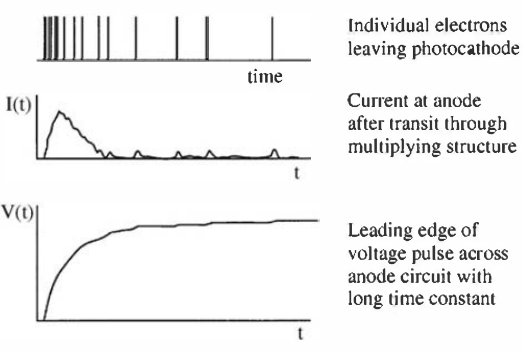
\includegraphics[scale=0.38]{fig47}
\end{figure}
\end{frame}

\section{Algunas cosas de las que no hablaré pero que valen la pena leer}

\begin{frame}
\begin{center}
 {\huge{\color{blue}Algunas cosas de las que no hablaré pero que valen la pena leer}} \\
 \vspace{0.5cm}
 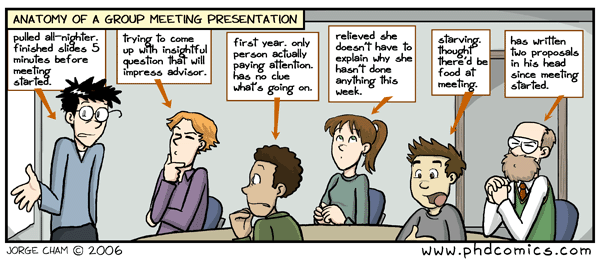
\includegraphics[scale=0.54]{fig48}
\end{center}
\end{frame}

\begin{frame}{Algunas cosas de las que no hablaré pero que valen la pena leer}
 \begin{itemize}
 \item \begin{justify}
        \textbf{Tubos FM híbridos}: La estructura fotomultiplicadora es reemplazada 
        por un detector de silicio. Uno de los beneficios más importantes es que 
        tienen un comportamiento estadístico superior de la amplificación  y 
        permiten separar eventos correspondientes a un solo fotoelectrón de 
        los eventos correspondientes a muchos fotoelectrones.
       \end{justify}
 \item \begin{justify}
        \textbf{Tubos FM detectores de posición}: Tubos FM que proveen información 
        de la posición de la luz incidente. Usan estructuras multiplicadoras que mantienen 
        la separación espacial entre las nubes de electrones que se originan de 
        los fotoelectrones generados en lugares separados del fotocátodo. También utilizan 
        dínodos especializados.
       \end{justify}
  \item \begin{justify}
        \textbf{Detectores de fotoionización}: Funcionan en el rango de la luz 
        ultravioleta. Vapor orgánico se incorpora como un componente del gas que 
        llena un detector convencional sensible a la ionización, entonces la amplitud 
        de la señal del pulso reflejará el número de fotones incidentes que se han 
        convertido en iones. Comúnmente se usan con tubos FM detectores de posición.
       \end{justify}
\end{itemize}
\end{frame}



\end{document}


